% !TeX root = ../main.tex
\chapter{Funzione di Eulero e gruppi}\label{cap:eulero-gruppi}
\fonti{Lezioni 16--24}

\section{La funzione di Eulero}
% A–L L16 p. 4; M–Z L15 pp. 10–11 e L16 pp. 2–4 (recupero D03).
Per contare gli invertibili nelle classi resto possiamo usare la scomposizione in prodotti di anelli. Il passaggio essenziale è che un isomorfismo trasporta esattamente gli elementi invertibili.

\begin{proposizione}\label{prop:trasporto-unita}
\begin{enumerate}[label=\arabic*.]
\item Se $f:R\to S$ è un morfismo e $a\in U(R)$, allora $f(a)\in U(S)$ e $f(a)^{-1}=f(a^{-1})$.
\item Se $f$ è un isomorfismo, la sua restrizione è una biezione $U(R)\to U(S)$.
\end{enumerate}
\end{proposizione}
\begin{proof}
\begin{enumerate}[label=\arabic*.]
\item Applicando $f$ alle identità $aa^{-1}=a^{-1}a=1_R$ si ottiene
\[
f(a)f(a^{-1})=f(a^{-1})f(a)=1_S.
\]
Quindi $f(a^{-1})$ è l'inverso di $f(a)$.
\item Se $f$ è un isomorfismo, anche $f^{-1}$ è un morfismo e manda $U(S)$ in $U(R)$: le due restrizioni sono inverse l'una dell'altra.
\end{enumerate}
\end{proof}

\begin{definizione}
La \textbf{funzione di Eulero} è
\[
\varphi:\N\setminus\{0,1\}\longrightarrow\N,\qquad
\varphi(m)=|U(\Z/m\Z)|.
\]
Per il criterio delle unità modulo $m$,
\[
\varphi(m)=\bigl|\{a\in\Z\mid 0\le a<m,\ \operatorname{MCD}(a,m)=1\}\bigr|.
\]
Conta dunque i rappresentanti coprimi con $m$ in un sistema completo di resti.
\end{definizione}

\begin{esempio}[Primi valori e cautele]
\[
\begin{array}{c|rrrrrrr}
m&2&3&4&5&6&7&8\\\hline
\varphi(m)&1&2&2&4&2&6&4
\end{array}
\]
Per esempio $U(\Z/8\Z)=\{[1]_8,[3]_8,[5]_8,[7]_8\}$, mentre le quattro unità modulo $12$ già elencate danno $\varphi(12)=4$.

La funzione non è monotona: $\varphi(5)=4>2=\varphi(6)$, ma $\varphi(6)=2<6=\varphi(7)$. Non conserva in generale né somme né prodotti: $\varphi(3+3)=2\ne4=\varphi(3)+\varphi(3)$ e $\varphi(2\cdot2)=2\ne1=\varphi(2)\varphi(2)$.
\end{esempio}

\begin{proposizione}\label{prop:eulero-potenze}
Per ogni primo positivo $p$ e ogni intero $k\ge1$,
\[
\varphi(p^k)=p^k-p^{k-1}=p^{k-1}(p-1).
\]
In particolare $\varphi(p)=p-1$ e $\varphi(p^2)=p^2-p$.
\end{proposizione}
\begin{proof}
Una classe $[a]_{p^k}$ è invertibile se e solo se $\operatorname{MCD}(a,p^k)=1$, cioè se e solo se $p\nmid a$: l'unico primo che divide $p^k$ è $p$. Fra i $p^k$ rappresentanti $0,1,\ldots,p^k-1$, quelli non invertibili sono precisamente
\[
0,p,2p,\ldots,(p^{k-1}-1)p.
\]
Sono $p^{k-1}$ multipli distinti di $p$, incluso lo zero. Restano $p^k-p^{k-1}$ unità. Per $k=1$ si esclude solo lo zero, come già sappiamo perché $\Z/p\Z$ è un campo.
\end{proof}

\Needspace{15\baselineskip}
\begin{proposizione}[Moltiplicatività per moduli coprimi]\label{prop:eulero-coprimi}
Se $m,n\ge2$ e $\operatorname{MCD}(m,n)=1$, allora
\[
\varphi(mn)=\varphi(m)\varphi(n).
\]
\end{proposizione}
\begin{proof}
Il teorema cinese dà l'isomorfismo $\Phi:\Z/mn\Z\to\Z/m\Z\times\Z/n\Z$. La proposizione~\ref{prop:trasporto-unita} e la descrizione delle unità di un prodotto danno una biezione
\[
U(\Z/mn\Z)\longrightarrow U(\Z/m\Z)\times U(\Z/n\Z),
\qquad [a]_{mn}\longmapsto([a]_m,[a]_n).
\]
Contando gli elementi dei due insiemi finiti si ottiene $\varphi(mn)=|U(\Z/m\Z)|\,|U(\Z/n\Z)|=\varphi(m)\varphi(n)$.
\end{proof}

\begin{corollario}[Formula dalla fattorizzazione]
% M–Z L16 p. 4; A–L L17 pp. 1–2 riprende la stessa prova e l'esempio600.
Se $m=p_1^{k_1}\cdots p_r^{k_r}\ge2$, con $p_i$ primi distinti e $k_i\ge1$, allora
\[
\varphi(m)=\prod_{i=1}^r p_i^{k_i-1}(p_i-1).
\]
\end{corollario}
\begin{proof}
Le potenze $p_i^{k_i}$ sono a due a due coprime, poiché hanno fattori primi distinti. Per il corollario~\ref{cor:crt-anelli}, la restrizione alle unità e la formula delle unità di un prodotto finito, si ha
\[
\varphi(m)=\prod_{i=1}^r\varphi(p_i^{k_i}).
\]
Applicando la proposizione~\ref{prop:eulero-potenze} a ciascun fattore segue la formula. Per $r=1$ è già la formula per una potenza prima.
\end{proof}

\begin{esempio}
Poiché $600=2^3\cdot3\cdot5^2$, con potenze prime a due a due coprime,
\[
\varphi(600)=\varphi(2^3)\varphi(3)\varphi(5^2)
           =\bigl(2^2(2-1)\bigr)\cdot(3-1)\cdot\bigl(5(5-1)\bigr)
           =4\cdot2\cdot20=160.
\]
\end{esempio}

% A–L L17 p. 2: esempi di unità, senza ripetere la formula o la prova.
\begin{esempio}[Unità modulo 3, 25 e 75]
Si ha $U(\Z/3\Z)=\{[1]_3,[2]_3\}$, mentre $U(\Z/25\Z)$ contiene le venti classi con rappresentante fra $0$ e $24$ non divisibile per $5$. Poiché $75=3\cdot25$, il teorema cinese dà una biezione fra $U(\Z/75\Z)$ e $U(\Z/3\Z)\times U(\Z/25\Z)$: una classe modulo $75$ è invertibile esattamente quando il suo rappresentante non è divisibile né per $3$ né per $5$. Quindi $\varphi(75)=2\cdot20=40$.
\end{esempio}

% !TeX root = ../main.tex
\section{Gruppi: assiomi e prime proprietà}
% A–L L17 pp. 3–6 e L18 p. 2; M–Z L17 pp. 1–3.
Un anello possiede due operazioni; un gruppo ne considera una sola. La struttura dipende sia dall'insieme sia dall'operazione scelta: gli interi sono un gruppo per la somma, ma non per il prodotto.

\begin{definizione}
Un \textbf{gruppo} è una coppia $(G,\cdot)$ con $G\ne\varnothing$ e un'operazione binaria $\cdot:G\times G\to G$ tale che:
\begin{enumerate}
\item $(ab)c=a(bc)$ per ogni $a,b,c\in G$;
\item esiste un \textbf{elemento neutro} $1_G\in G$ con $1_Ga=a1_G=a$ per ogni $a\in G$;
\item per ogni $a\in G$ esiste un \textbf{inverso} $b\in G$ con $ab=ba=1_G$.
\end{enumerate}
Il gruppo è \textbf{abeliano}, o \textbf{commutativo}, se inoltre $ab=ba$ per ogni $a,b\in G$. Il prodotto $ab$ abbrevia $a\cdot b$; la commutatività non è richiesta negli assiomi di gruppo.
\end{definizione}

\begin{proposizione}\label{prop:gruppo-prime}
In un gruppo valgono:
\begin{enumerate}[label=\arabic*.]
\item Il neutro e l\textquotesingle inverso di ciascun elemento sono unici. Indicato l\textquotesingle inverso di $a$ con $a^{-1}$, si ha $(a^{-1})^{-1}=a$.
\item $ac=bc\Rightarrow a=b$ e $ca=cb\Rightarrow a=b$ (cancellazione).
\item $(ab)^{-1}=b^{-1}a^{-1}$.
\end{enumerate}
\end{proposizione}
\begin{proof}
\begin{enumerate}[label=\arabic*.]
\item Se $e,e'$ sono neutri, $e=ee'=e'$. Se $b,c$ sono inversi di $a$, allora $b=b(ac)=(ba)c=c$. Le identità $aa^{-1}=a^{-1}a=1_G$ mostrano anche che $a$ è l'inverso di $a^{-1}$.
\item Da $ac=bc$ si ottiene $(ac)c^{-1}=(bc)c^{-1}$ e, per associatività, $a=b$. Da $ca=cb$ si moltiplica invece a sinistra per $c^{-1}$. Non si scambia l'ordine dei fattori.
\item Infine
\[
(ab)(b^{-1}a^{-1})=a(bb^{-1})a^{-1}=1_G,
\qquad (b^{-1}a^{-1})(ab)=b^{-1}(a^{-1}a)b=1_G.
\]
L'unicità dell'inverso dà la formula per $(ab)^{-1}$: occorre invertire anche l'ordine.
\end{enumerate}
\end{proof}

\subsection{Potenze e notazione additiva}
\begin{definizione}
Per $a\in G$ e $n\ge1$, $a^n$ è il prodotto di $n$ fattori uguali ad $a$. Si pone inoltre
\[
a^0=1_G,\qquad a^{-n}=(a^{-1})^n\quad(n\ge1).
\]
In un gruppo abeliano si può usare la \textbf{notazione additiva}: l'operazione si scrive $+$, il neutro $0$, l'inverso di $a$ si scrive $-a$, e la potenza $a^n$ diventa il multiplo $na$. Per esempio, in $(\Z,+)$, $3a=a+a+a$.
\end{definizione}

\begin{proposizione}\label{prop:potenze-gruppo}
Per ogni $a\in G$ e $m,n\in\Z$,
\begin{enumerate}[label=\arabic*.]
\item $a^ma^n=a^{m+n}$.
\item $(a^n)^{-1}=a^{-n}$.
\item $(a^m)^n=a^{mn}$.
\end{enumerate}
In particolare due potenze dello stesso elemento commutano, anche se $G$ non è abeliano.
\end{proposizione}
\begin{proof}
\begin{enumerate}[label=\arabic*.]
\item La concatenazione dei fattori dà la prima identità per $m,n\ge0$. Ripetendo la formula dell'inverso di un prodotto si ha $(a^k)^{-1}=(a^{-1})^k$ per $k\ge1$.

Se $m\ge0$ e $n=-k<0$, per $m\ge k$ si scrive $a^m=a^{m-k}a^k$ e si cancella $a^k$ con $(a^k)^{-1}$. Per $m<k$ si scrive $a^k=a^{k-m}a^m$, quindi $a^m(a^k)^{-1}=(a^{k-m})^{-1}=a^{m-k}$. Il caso $m<0,n\ge0$ si ottiene con le stesse cancellazioni sull'altro lato. Se entrambi sono negativi, si applica la concatenazione alle potenze di $a^{-1}$. La formula vale così per tutti gli interi.
\item Ponendo $m=-n$ nel punto~1 si verifica l'identità sull'inverso.
\item Fissato $m\in\Z$, per $n=0$ entrambi i membri valgono $1_G$. Se la formula vale per $n\ge0$, allora
\[
(a^m)^{n+1}=(a^m)^na^m=a^{mn}a^m=a^{m(n+1)}
\]
per il punto~1. L'induzione dà il risultato per ogni $n\ge0$. Se $n=-k<0$, la definizione, il caso non negativo e il punto~2 danno $(a^m)^{-k}=((a^m)^k)^{-1}=(a^{mk})^{-1}=a^{-mk}$.
\end{enumerate}
Infine $m+n=n+m$ nel punto~1 dà la commutazione delle potenze di $a$.
\end{proof}

\subsection{Gruppi ottenuti dagli anelli}
\begin{proposizione}
\begin{enumerate}[label=\arabic*.]
\item Se $R$ è un anello, $(R,+)$ è un gruppo abeliano.
\item Se $R$ ha unità, $(U(R),\cdot)$ è un gruppo, abeliano quando $R$ è commutativo.
\item Se $K$ è un campo, $U(K)=K\setminus\{0\}$.
\end{enumerate}
\end{proposizione}
\begin{proof}
\begin{enumerate}[label=\arabic*.]
\item Gli assiomi additivi di anello sono esattamente quelli di un gruppo abeliano.
\item Per il prodotto delle unità, l'operazione è interna perché, per $a,b\in U(R)$, $b^{-1}a^{-1}$ è un inverso bilatero di $ab$. L'associatività è ereditata da $R$, $1_R$ è invertibile e l'inverso di un'unità è ancora un'unità. Se $R$ è commutativo lo è anche il prodotto ristretto.
\item In un campo ogni elemento non nullo è invertibile, mentre lo zero non lo è perché $1_K\ne0_K$.
\end{enumerate}
\end{proof}

\begin{esempio}
$(\Z,+)$, $(\Z/25\Z,+)$ e $(U(\Z/25\Z),\cdot)$ sono gruppi abeliani. I due gruppi modulo $25$ hanno rispettivamente $25$ e $20$ elementi: cambiano sia l'insieme sia l'operazione. In generale $U(\Z/m\Z)$ ha $\varphi(m)$ elementi. Poiché $13$ è primo, $U(\Z/13\Z)$ è il gruppo moltiplicativo delle dodici classi non nulle.

$(\Z,\cdot)$, $(\Q,\cdot)$ e $(\R,\cdot)$ non sono gruppi: contengono lo zero, che non ha inverso moltiplicativo. Sono invece gruppi abeliani $(\Q\setminus\{0\},\cdot)$ e $(\R\setminus\{0\},\cdot)$.
\end{esempio}

\section{Permutazioni e trasformazioni affini}
\subsection{Il gruppo simmetrico}
% A–L L17 pp. 7–8; M–Z L17 pp. 3–5.
Le operazioni puntuali sulle funzioni e la composizione sono operazioni diverse. Nell'anello $\R^{\R}$ con prodotto puntuale, le unità sono le funzioni che non si annullano mai e formano un gruppo abeliano; per la composizione, invece, le funzioni invertibili sono esattamente le biezioni. Tutte le funzioni $\R\to\R$ con la sola composizione formano un monoide: la composizione è associativa e ha neutro $\operatorname{id}_{\R}$, ma non tutte le funzioni hanno inversa.

\begin{definizione}
Per un insieme non vuoto $X$, si indica con
\[
S_X=\operatorname{Sym}(X)=\operatorname{Perm}(X)
   =\{\sigma:X\to X\mid\sigma\text{ è biettiva}\}
\]
l'insieme delle \textbf{permutazioni} di $X$. Con la composizione forma il \textbf{gruppo simmetrico} su $X$. Se $X=\{1,\ldots,n\}$, si scrive $S_n$.
\end{definizione}

\begin{proposizione}\label{prop:simmetrico}
\begin{enumerate}[label=\arabic*.]
\item $S_X$ è un gruppo con neutro $\operatorname{id}_X$ e inversa la funzione inversa.
\item Per $n\ge1$, $|S_n|=n!$.
\item Se $X$ ha almeno tre elementi, $S_X$ non è abeliano.
\end{enumerate}
\end{proposizione}
\begin{proof}
\begin{enumerate}[label=\arabic*.]
\item La composta di due biezioni è biettiva; la composizione è associativa, l'identità è biettiva e l'inversa di una biezione è biettiva. Sono le proprietà già dimostrate per le funzioni.
\item Per scegliere una biezione di $\{1,\ldots,n\}$, l'immagine di $1$ ha $n$ possibilità, quella di $2$ ne ha $n-1$ perché deve essere diversa, e così via fino all'ultima scelta obbligata. Il conteggio è $n(n-1)\cdots1=n!$.
\item Scelti tre punti distinti $x,y,z$, siano $s$ lo scambio di $x,y$ e $t$ lo scambio di $y,z$, lasciando fissi gli altri punti. Allora $(s\circ t)(x)=y$, mentre $(t\circ s)(x)=z$: le due composte sono diverse. Per uno o due punti, invece, il gruppo è abeliano (rispettivamente il solo neutro, oppure neutro e unico scambio).
\end{enumerate}
\end{proof}

\Needspace{30\baselineskip}
\begin{esempio}[Leggere e comporre le permutazioni]
La notazione su due righe elenca sopra gli argomenti e sotto le immagini. In $S_4$, siano
\[
\sigma=\begin{pmatrix}1&2&3&4\\1&3&2&4\end{pmatrix},\qquad
\tau=\begin{pmatrix}1&2&3&4\\4&2&1&3\end{pmatrix}.
\]
Si ha $\sigma^2=\operatorname{id}$, quindi $\sigma^{-1}=\sigma$. Nella composta $\sigma\circ\tau$ si applica prima $\tau$, poi $\sigma$:
\[
\begin{array}{c|rrrr}
x&1&2&3&4\\\hline
\tau(x)&4&2&1&3\\
\sigma(\tau(x))&4&3&1&2
\end{array}
\]
Per seguire un singolo punto, il percorso è
\begin{center}
\begin{tikzpicture}[>=Stealth,baseline]
\node (a) at (0,0) {$2$}; \node (b) at (2.2,0) {$2$}; \node (c) at (4.4,0) {$3$};
\draw[->] (a)--node[above]{$\tau$}(b); \draw[->] (b)--node[above]{$\sigma$}(c);
\end{tikzpicture}
\end{center}
Invertendo l'ordine si ottiene invece
\[
\sigma\circ\tau=\begin{pmatrix}1&2&3&4\\4&3&1&2\end{pmatrix},\qquad
\tau\circ\sigma=\begin{pmatrix}1&2&3&4\\4&1&2&3\end{pmatrix}.
\]
Un secondo esempio, con $\rho=\left(\begin{smallmatrix}1&2&3&4\\3&2&4&1\end{smallmatrix}\right)$, dà
\[
\rho\circ\sigma=\begin{pmatrix}1&2&3&4\\3&4&2&1\end{pmatrix},\qquad
\sigma\circ\rho=\begin{pmatrix}1&2&3&4\\2&3&4&1\end{pmatrix}.
\]
Anche qui l'ordine delle applicazioni modifica il risultato.
\end{esempio}

\subsection{Il gruppo affine reale}
% A–L L17 pp. 9–10 e L18 p. 1 (pagina ripetuta); M–Z L17 pp. 5–6.
\begin{definizione}
Per $a\in\R\setminus\{0\}$ e $b\in\R$, poniamo $f_{a,b}(x)=ax+b$. L'insieme
\[
\operatorname{Aff}(\R)=\{f_{a,b}:\R\to\R\mid a\ne0,\ b\in\R\}
\]
è l'insieme delle \textbf{trasformazioni affini reali invertibili}; lo consideriamo con la composizione. I coefficienti sono univoci: $b=f_{a,b}(0)$ e $a=f_{a,b}(1)-f_{a,b}(0)$.
\end{definizione}

\begin{proposizione}\label{prop:affini}
\begin{enumerate}[label=\arabic*.]
\item $\operatorname{Aff}(\R)$ è un gruppo non abeliano e
\[
f_{a,b}\circ f_{a',b'}=f_{aa',\,ab'+b},\qquad
1_{\operatorname{Aff}(\R)}=f_{1,0},\qquad
f_{a,b}^{-1}=f_{a^{-1},\,-ba^{-1}}.
\]
\item Due trasformazioni $f_{a,b}$ e $f_{a',b'}$ commutano se e solo se
\[
(1-a')b=(1-a)b'.
\]
\end{enumerate}
\end{proposizione}
\begin{proof}
\begin{enumerate}[label=\arabic*.]
\item Applicando prima $f_{a',b'}$ e poi $f_{a,b}$ si ottiene $a(a'x+b')+b=aa'x+ab'+b$. Poiché $aa'\ne0$, la composizione appartiene ancora all'insieme. L'associatività è quella della composizione di funzioni e $f_{1,0}$ è l'identità. Risolvendo $y=ax+b$ si trova $x=a^{-1}y-ba^{-1}$; sostituendo, questa funzione è inversa su entrambi i lati. Quindi ogni elemento è una biezione e gli assiomi di gruppo sono verificati.
\item Le due composte hanno lo stesso coefficiente $aa'=a'a$; coincidono se e solo se $ab'+b=a'b+b'$, equivalente al criterio enunciato. Non vale per ogni coppia: $f_{2,1}\circ f_{1,2}$ manda $x$ in $2x+5$, mentre $f_{1,2}\circ f_{2,1}$ lo manda in $2x+3$.
\end{enumerate}
\end{proof}

% !TeX root = ../main.tex
\section{Sottogruppi e sottogruppi generati}
% A–L L18 pp. 2–5; M–Z L17 p. 7 e L18 pp. 1–3.
\begin{definizione}
Un \textbf{sottogruppo} di un gruppo $G$ è un sottoinsieme non vuoto $H\subseteq G$ tale che la restrizione dell'operazione di $G$ definisca su $H$ una struttura di gruppo. Si scrive $H\le G$. La restrizione deve essere un'operazione $H\times H\to H$: per ogni $h,k\in H$ deve quindi risultare $hk\in H$.
\end{definizione}

\begin{proposizione}[Criteri di sottogruppo]\label{prop:criterio-sottogruppo}
Per $\varnothing\ne H\subseteq G$, sono equivalenti:
\begin{enumerate}
\item $H\le G$;
\item per ogni $h,k\in H$, $hk\in H$, e per ogni $h\in H$, $h^{-1}\in H$;
\item per ogni $h,k\in H$, $hk^{-1}\in H$.
\end{enumerate}
In tal caso il neutro di $H$ è $1_G$ e l'inverso di un elemento in $H$ coincide con quello calcolato in $G$.
\end{proposizione}
\begin{proof}
\textbf{1 implica 2.} Sia $e_H$ il neutro di $H$. Scelto $h\in H$, da $he_H=h=h1_G$ e dalla cancellazione in $G$ segue $e_H=1_G$. L'inverso in $H$ è dunque anche inverso in $G$, e coincide con $h^{-1}$ per unicità. La chiusura del prodotto è parte della definizione.

\textbf{2 implica 1.} Scelto $h\in H$, le due chiusure danno $1_G=hh^{-1}\in H$. Associatività, neutro e inversi sono quelli di $G$, e valgono anche sugli elementi di $H$.

\textbf{2 implica 3.} Si applicano in successione la chiusura rispetto all'inverso e quella rispetto al prodotto.

\textbf{3 implica 2.} Per $h\in H$, $hh^{-1}=1_G\in H$. Quindi, per ogni $k\in H$, $1_Gk^{-1}=k^{-1}\in H$; infine $hk=h(k^{-1})^{-1}\in H$. La condizione $H\ne\varnothing$ serve per partire da un suo elemento.
\end{proof}

\subsection{Intersezioni, unioni ed estremo superiore}
\begin{proposizione}\label{prop:intersezione-sottogruppi}
\begin{enumerate}[label=\arabic*.]
\item L'intersezione di una famiglia non vuota di sottogruppi di $G$ è un sottogruppo. In particolare $H_1\cap H_2$ è il più grande sottogruppo contenuto sia in $H_1$ sia in $H_2$.
\item Anche $\{1_G\}$ e $G$ sono sottogruppi di $G$.
\end{enumerate}
\end{proposizione}
\begin{proof}
\begin{enumerate}[label=\arabic*.]
\item Il neutro appartiene a tutti i sottogruppi, quindi all'intersezione. Se $h,k$ appartengono all'intersezione, $hk^{-1}$ appartiene a ogni sottogruppo della famiglia, dunque ancora all'intersezione. Si applica il criterio precedente. Ogni sottogruppo contenuto nei due fattori è contenuto nella loro intersezione, che è quindi il più grande fra questi.
\item Per $\{1_G\}$ e $G$ lo stesso criterio si verifica direttamente.
\end{enumerate}
\end{proof}

\begin{proposizione}\label{prop:unione-sottogruppi}
Per $H_1,H_2\le G$, l'unione $H_1\cup H_2$ è un sottogruppo se e solo se $H_1\subseteq H_2$ oppure $H_2\subseteq H_1$.
\end{proposizione}
\begin{proof}
Se uno dei due contiene l'altro, l'unione coincide con il più grande ed è un sottogruppo. Viceversa, se nessuno contiene l'altro, scegliamo $a\in H_1\setminus H_2$ e $b\in H_2\setminus H_1$. Se l'unione fosse un sottogruppo, conterrebbe $ab$. Se $ab\in H_1$, allora $b=a^{-1}(ab)\in H_1$, assurdo. Se $ab\in H_2$, allora $a=(ab)b^{-1}\in H_2$, ancora assurdo. Le due possibilità esauriscono l'unione.
\end{proof}

% A–L L19 pp. 1–3; M–Z L19 pp. 1–2: generalizzazione integrata qui.
\begin{definizione}
Per $X\subseteq G$, il \textbf{sottogruppo generato da $X$} è
\[
\langle X\rangle=\bigcap\{H\le G\mid X\subseteq H\}.
\]
La famiglia contiene $G$, quindi è non vuota; la sua intersezione è un sottogruppo che contiene $X$ ed è contenuto in ogni sottogruppo contenente $X$. È dunque il più piccolo sottogruppo contenente $X$. Gli elementi di $X$ si chiamano \textbf{generatori} di $\langle X\rangle$; si scrive anche $\langle x_1,\ldots,x_r\rangle$ quando $X=\{x_1,\ldots,x_r\}$. In particolare $\langle\varnothing\rangle=\{1_G\}$.
\end{definizione}

\begin{proposizione}[Descrizione mediante parole]\label{prop:generato-parole}
Sia $X\subseteq G$.
\begin{enumerate}[label=\arabic*.]
\item $\langle X\rangle$ è l'insieme dei prodotti finiti
\[
x_1^{\varepsilon_1}\cdots x_r^{\varepsilon_r},\qquad
r\in\N,\quad x_i\in X,\quad\varepsilon_i\in\{1,-1\}.
\]
Il prodotto con $r=0$, detto \emph{parola vuota}, vale $1_G$.
\item Se $G$ è abeliano, gli stessi elementi si possono scrivere come prodotti finiti $x_1^{n_1}\cdots x_r^{n_r}$ con $n_i\in\Z$. In notazione additiva sono le combinazioni intere finite $n_1x_1+\cdots+n_rx_r$.
\end{enumerate}
\end{proposizione}
\begin{proof}
\begin{enumerate}[label=\arabic*.]
\item Indichiamo con $W$ l'insieme delle parole descritte. Contiene $1_G$; il prodotto di due parole è la loro concatenazione, quindi appartiene a $W$. Inoltre
\[
(x_1^{\varepsilon_1}\cdots x_r^{\varepsilon_r})^{-1}
=x_r^{-\varepsilon_r}\cdots x_1^{-\varepsilon_1}\in W.
\]
Quindi $W\le G$ e contiene $X$, da cui $\langle X\rangle\subseteq W$. Viceversa ogni sottogruppo contenente $X$ contiene gli inversi delle sue lettere e tutti i loro prodotti finiti: contiene dunque $W$. Applicando questo a $\langle X\rangle$ si ottiene $W\subseteq\langle X\rangle$. Per $X=\varnothing$ resta soltanto la parola vuota.
\item Se il prodotto è commutativo, si possono riordinare le lettere di una parola e raccogliere quelle uguali in potenze intere. Viceversa ogni potenza intera è un prodotto di lettere o dei loro inversi (oppure il prodotto vuoto). In notazione additiva il prodotto diventa somma e la potenza $x^n$ diventa $nx$.
\end{enumerate}
\end{proof}

La scrittura mediante parole non è in generale unica: per esempio, se $x_1=x_2x_3$, un elemento ha già due espressioni diverse. Nei gruppi non abeliani l'ordine dei fattori va conservato. Se $\sigma\in S_{10}$ manda $1\mapsto2\mapsto3\mapsto1$ e fissa gli altri punti, allora $\sigma^3=\operatorname{id}$. Per ogni $\tau\in S_{10}$,
\[
\sigma\sigma\sigma\tau=\tau,\qquad
\sigma\tau\sigma^3\tau=\sigma\tau^2.
\]
Si cancellano blocchi adiacenti, senza scambiare arbitrariamente $\sigma$ e $\tau$.

\begin{definizione}
Per $H_1,H_2\le G$, il \textbf{sottogruppo generato da $H_1$ e $H_2$}, indicato con $\langle H_1,H_2\rangle$ o $H_1\vee H_2$, è $\langle H_1\cup H_2\rangle$, cioè
\[
H_1\vee H_2=\bigcap\{H\le G\mid H_1\cup H_2\subseteq H\}.
\]
La famiglia è non vuota perché contiene $G$; l'intersezione è un sottogruppo e contiene entrambi. Per costruzione è il \emph{più piccolo} sottogruppo che li contiene: è l'estremo superiore per l'inclusione, mentre $H_1\cap H_2$ è l'estremo inferiore.
\end{definizione}

\begin{center}
\begin{tikzpicture}[>=Stealth]
\node (b) at (0,0) {$H_1\cap H_2$};
\node (l) at (-2,1.25) {$H_1$}; \node (r) at (2,1.25) {$H_2$};
\node (t) at (0,2.5) {$H_1\vee H_2$};
\draw[->] (b)--(l); \draw[->] (b)--(r); \draw[->] (l)--(t); \draw[->] (r)--(t);
\end{tikzpicture}
\end{center}
Le frecce indicano inclusioni dal basso verso l'alto; alcuni nodi possono coincidere. L'unione insiemistica è contenuta nel sottogruppo generato, ma in generale non coincide con esso.

\subsection{Esempi nelle trasformazioni affini e nelle permutazioni}
Richiamiamo $f_{a,b}(x)=ax+b$ con $a\ne0$, e il prodotto dato dalla composizione. In $\operatorname{Aff}(\R)$ consideriamo
\[
\mathcal O=\{f_{a,0}\mid a\in\R\setminus\{0\}\},\qquad
\mathcal T=\{f_{1,b}\mid b\in\R\}.
\]
Sono rispettivamente le \textbf{omotetie con centro nell'origine} (inclusi i rapporti negativi) e le \textbf{traslazioni}.

\begin{proposizione}\label{prop:sottogruppi-affini}
\begin{enumerate}[label=\arabic*.]
\item $\mathcal O$ e $\mathcal T$ sono sottogruppi abeliani di $\operatorname{Aff}(\R)$; inoltre
\[
\mathcal O\cap\mathcal T=\{f_{1,0}\},\qquad
\mathcal O\vee\mathcal T=\operatorname{Aff}(\R).
\]
\item Sono sottogruppi anche
\[
H=\{f_{a,b}\mid a\in\Q\setminus\{0\},\ b\in\R\},\qquad
\operatorname{Aff}(\Q)=\{f_{a,b}\mid a\in\Q\setminus\{0\},\ b\in\Q\},
\]
qui entrambi considerati come insiemi di funzioni $\R\to\R$.
\end{enumerate}
\end{proposizione}
\begin{proof}
\begin{enumerate}[label=\arabic*.]
\item Per le omotetie, $f_{a,0}\circ f_{c,0}=f_{ac,0}$ e $f_{a,0}^{-1}=f_{1/a,0}$. Per le traslazioni, $f_{1,b}\circ f_{1,d}=f_{1,b+d}$ e $f_{1,b}^{-1}=f_{1,-b}$. Entrambi gli insiemi contengono $f_{1,0}$, sono chiusi e hanno operazione commutativa perché $ac=ca$ e $b+d=d+b$.

Un'affinità è in entrambi esattamente quando $a=1,b=0$. Ogni affinità si scrive invece $f_{a,b}=f_{1,b}\circ f_{a,0}$, prodotto di una traslazione e un'omotetia. Ogni sottogruppo che contiene $\mathcal O$ e $\mathcal T$ contiene quindi tutte le affinità: il loro generato è l'intero gruppo, che non è abeliano pur essendolo i due sottogruppi.
\item Per $H$, prodotto e inverso hanno ancora pendenza razionale non nulla: $ac\in\Q\setminus\{0\}$ e $1/a\in\Q\setminus\{0\}$, mentre i termini noti possono essere reali. Per $\operatorname{Aff}(\Q)$, le formule $ad+b$ e $-b/a$ conservano anche la razionalità del termine noto. Il criterio di sottogruppo si applica a entrambi. I due esempi sono distinti: $f_{1,\sqrt2}$ appartiene a $H$, ma non a $\operatorname{Aff}(\Q)$. Inoltre $\mathcal T\subsetneq H$, perché $f_{2,0}\in H\setminus\mathcal T$, e $H\ne\mathcal O$, perché $f_{1,1}\in H\setminus\mathcal O$.
\end{enumerate}
\end{proof}

\begin{esempio}[Permutazioni che fissano dei punti]
Per $\varnothing\ne X_0\subseteq X$, l'insieme
\[
\operatorname{Fix}(X_0)=\{\sigma\in S_X\mid\sigma(x)=x\text{ per ogni }x\in X_0\}
\]
è un sottogruppo: contiene l'identità; se $\sigma,\tau$ fissano ogni $x\in X_0$, $(\sigma\circ\tau)(x)=\sigma(x)=x$; da $\sigma(x)=x$, applicando $\sigma^{-1}$ si ricava $\sigma^{-1}(x)=x$. Si tratta di fissare ogni punto singolarmente, non soltanto di mandare $X_0$ in se stesso. Per $X_0=\{x_0\}$ si ottiene il sottogruppo delle permutazioni che fissano il punto $x_0$.
\end{esempio}

\subsection{Il sottogruppo ciclico generato da un elemento}
\begin{proposizione}\label{prop:ciclico}
Per $g\in G$, l'insieme
\[
\langle g\rangle=\{g^n\mid n\in\Z\}
\]
ha le seguenti proprietà:
\begin{enumerate}[label=\arabic*.]
\item è un sottogruppo abeliano;
\item è il più piccolo sottogruppo di $G$ contenente $g$.
\end{enumerate}
Si chiama \textbf{sottogruppo ciclico generato da $g$}.
\end{proposizione}
\begin{proof}
\begin{enumerate}[label=\arabic*.]
\item Contiene $1_G=g^0$; per la proposizione~\ref{prop:potenze-gruppo}, $g^mg^n=g^{m+n}$ e $(g^n)^{-1}=g^{-n}$, dunque è un sottogruppo. È abeliano perché $m+n=n+m$.
\item Se $H\le G$ contiene $g$, contiene $g^{-1}$ e tutti i loro prodotti finiti, quindi tutte le potenze intere di $g$. Perciò $\langle g\rangle\subseteq H$.
\end{enumerate}
\end{proof}

\begin{esempio}
In notazione additiva, $\langle g\rangle=\{ng\mid n\in\Z\}$. In $(\Z,+)$ si ha quindi $\langle3\rangle=3\Z$ e, più in generale, $\langle m\rangle=m\Z$ per $m\in\Z$; per $m=0$ si ottiene il sottogruppo $\{0\}$.
\end{esempio}

\Needspace{11\baselineskip}
\begin{esercizio}
In $S_5$, determinare tutti gli elementi di $\langle\pi\rangle$ per
$\pi=\left(\begin{smallmatrix}1&2&3&4&5\\4&3&1&2&5\end{smallmatrix}\right)$.
\end{esercizio}
\begin{svolgimento}
Componendo la permutazione con se stessa si trova
\[
\pi^2=\begin{pmatrix}1&2&3&4&5\\2&1&4&3&5\end{pmatrix},\qquad
\pi^3=\begin{pmatrix}1&2&3&4&5\\3&4&2&1&5\end{pmatrix},\qquad
\pi^4=\operatorname{id}.
\]
Le quattro permutazioni $\operatorname{id},\pi,\pi^2,\pi^3$ sono distinte. Ogni esponente intero si riduce modulo $4$, perché $\pi^4=1$ e anche $\pi^{-1}=\pi^3$. Dunque sono tutti e soli gli elementi di $\langle\pi\rangle$.
\end{svolgimento}

\Needspace{23\baselineskip}
\subsection{Tutti i sottogruppi degli interi}
% A–L L19 pp. 4–5; M–Z L19 pp. 3–4.
\begin{proposizione}\label{prop:sottogruppi-Z}
Ogni sottogruppo di $(\Z,+)$ è $m\Z$ per un unico $m\in\N$.
\end{proposizione}
\begin{proof}
Se $H=\{0\}$, si prende $m=0$. Se $H\ne\{0\}$, contiene un intero non nullo e il suo opposto, dunque contiene un positivo. Per buon ordinamento esiste
\[
m=\min(H\cap\N^*)>0.
\]
Poiché $m\in H$, tutti i suoi multipli interi appartengono a $H$, quindi $m\Z\subseteq H$. Per $n\in H$, la divisione euclidea dà $n=mq+r$, con $q\in\Z$ e $0\le r<m$. Ma $r=n-mq\in H$: se fosse positivo contraddirebbe la scelta di $m$. Quindi $r=0$ e $n\in m\Z$, da cui l'inclusione opposta. L'unicità segue perché per un sottogruppo non nullo $m$ è il suo minimo elemento positivo; $0\Z$ è invece l'unico caso senza positivi.
\end{proof}

\Needspace{12\baselineskip}
\begin{proposizione}\label{prop:reticolo-Z}
\begin{enumerate}[label=\arabic*.]
\item Per $m,n\in\N$, $m\Z\subseteq n\Z$ se e solo se $n\mid m$.
\item Per $m,n>0$,
\[
m\Z\vee n\Z=\langle m,n\rangle=\operatorname{MCD}(m,n)\Z,
\qquad m\Z\cap n\Z=\operatorname{mcm}(m,n)\Z.
\]
\end{enumerate}
\end{proposizione}
\begin{proof}
\begin{enumerate}[label=\arabic*.]
\item L'inclusione implica $m\in n\Z$, quindi $n\mid m$. Viceversa, se $m=nq$, ogni multiplo $mk=n(qk)$ appartiene a $n\Z$. Il ragionamento comprende lo zero: $0$ divide soltanto $0$.
\item Un sottogruppo contiene $m,n$ esattamente quando contiene $m\Z,n\Z$, dunque i due generati coincidono. Nel gruppo abeliano $(\Z,+)$ essi sono l'insieme delle combinazioni $am+bn$, con $a,b\in\Z$. Posto $d=\operatorname{MCD}(m,n)$, ciascuna combinazione è multipla di $d$; viceversa Bézout dà una combinazione uguale a $d$, quindi il generato contiene tutti i multipli di $d$. L'intersezione consiste invece negli interi multipli sia di $m$ sia di $n$: per la caratterizzazione aritmetica del minimo comune multiplo sono esattamente i multipli di $\operatorname{mcm}(m,n)$, incluso zero e i negativi.
\end{enumerate}
\end{proof}

\begin{esempio}[MCD, mcm e inclusione]
Si ha $m\Z=(-m)\Z$ per ogni intero $m$. Per $m=12$ e $n=21$,
\[
12\Z\vee21\Z=3\Z,\qquad12\Z\cap21\Z=84\Z.
\]
Per $m,n>0$ le inclusioni si dispongono come nel diagramma seguente; le frecce vanno dal sottogruppo contenuto a quello contenente e alcuni nodi possono coincidere.
\begin{center}
\begin{tikzpicture}[>=Stealth]
\node (z) at (0,4.5) {$\Z$};
\node (d) at (0,3.6) {$\operatorname{MCD}(m,n)\Z$};
\node (m) at (-2.1,2.5) {$m\Z$}; \node (n) at (2.1,2.5) {$n\Z$};
\node (l) at (0,1.3) {$\operatorname{mcm}(m,n)\Z$};
\node (o) at (0,.2) {$\{0\}$};
\draw[->] (o)--(l); \draw[->] (l)--(m); \draw[->] (l)--(n);
\draw[->] (m)--(d); \draw[->] (n)--(d); \draw[->] (d)--(z);
\end{tikzpicture}
\end{center}
\end{esempio}

\Needspace{12\baselineskip}
\begin{esercizio}
Determinare tutti i sottogruppi di $(\Z,+)$ contenenti $12\Z$ e disegnarne il reticolo delle inclusioni.
\end{esercizio}
\begin{svolgimento}
Ogni sottogruppo è $m\Z$, con $m\ge0$, e $12\Z\subseteq m\Z$ equivale a $m\mid12$. I soli valori sono $1,2,3,4,6,12$; il valore $0$ non è ammesso perché $12\notin\{0\}$.
\begin{center}
\begin{tikzpicture}[>=Stealth]
\node (a) at (0,3.4) {$\Z$};
\node (b) at (-1.9,2.3) {$2\Z$}; \node (c) at (1.9,2.3) {$3\Z$};
\node (d) at (-1.9,1.2) {$4\Z$}; \node (e) at (1.9,1.2) {$6\Z$};
\node (f) at (0,.1) {$12\Z$};
\draw[->] (f)--(d); \draw[->] (f)--(e); \draw[->] (d)--(b);
\draw[->] (e)--(b); \draw[->] (e)--(c); \draw[->] (b)--(a); \draw[->] (c)--(a);
\end{tikzpicture}
\end{center}
Le frecce rappresentano inclusioni dal basso verso l'alto; tutte le altre inclusioni si ottengono per transitività.
\end{svolgimento}


% !TeX root = ../main.tex
\section{Coniugati, centralizzanti e centro}
% A–L L18 pp. 6–8; M–Z L18 pp. 4–6.
\begin{definizione}
Per $a,b\in G$, il \textbf{coniugato di $b$ tramite $a$} è
\[
b^a:=aba^{-1}.
\]
Qui l'esponente è un elemento del gruppo e indica un coniugato; non è la potenza intera $b^n$. Moltiplicando a destra per $a$ si vede che
\[
ab=ba\quad\Longleftrightarrow\quad aba^{-1}=b\quad\Longleftrightarrow\quad b^a=b.
\]
Quindi $G$ è abeliano se e solo se ogni coniugato di ogni elemento coincide con l'elemento stesso.
\end{definizione}

\begin{esempio}[Coniugati nel gruppo affine]
Per una traslazione $f_{1,b}$ e un'omotetia $f_{a,0}$, con $a\ne0$,
\[
(f_{1,b})^{f_{a,0}}=f_{a,0}\circ f_{1,b}\circ f_{1/a,0}=f_{1,ab}.
\]
Il percorso $x\mapsto x/a\mapsto x/a+b\mapsto x+ab$ dà ancora una traslazione; coincide con $f_{1,b}$ se e solo se $(a-1)b=0$.

Invertendo i ruoli, invece,
\[
(f_{a,0})^{f_{1,b}}=f_{1,b}\circ f_{a,0}\circ f_{1,-b}=f_{a,\,b(1-a)}.
\]
Infatti $x\mapsto x-b\mapsto a(x-b)\mapsto ax+b(1-a)$. In generale il termine noto non è nullo, quindi il risultato non è un'omotetia con centro nell'origine.
\end{esempio}

\Needspace{12\baselineskip}
\begin{esercizio}
In $S_4$, per
\[
s=\begin{pmatrix}1&2&3&4\\2&3&4&1\end{pmatrix},\qquad
t=\begin{pmatrix}1&2&3&4\\1&4&3&2\end{pmatrix},
\]
calcolare i coniugati $s^t$ e $t^s$.
\end{esercizio}
\begin{svolgimento}
Si calcolano $s^t=t\circ s\circ t^{-1}$ e $t^s=s\circ t\circ s^{-1}$, sempre applicando per prima la funzione più a destra. Qui $t^{-1}=t$ e $s^{-1}=\left(\begin{smallmatrix}1&2&3&4\\4&1&2&3\end{smallmatrix}\right)$. Seguendo i quattro argomenti si ottiene
\[
s^t=\begin{pmatrix}1&2&3&4\\4&1&2&3\end{pmatrix},\qquad
t^s=\begin{pmatrix}1&2&3&4\\3&2&1&4\end{pmatrix}.
\]
Per esempio $s^t(1)=t(s(t^{-1}(1)))=t(s(1))=t(2)=4$.
\end{svolgimento}

\Needspace{18\baselineskip}
\subsection{Gli elementi che commutano}
\begin{definizione}
Per $x\in G$, il \textbf{centralizzante} di $x$ in $G$ è
\[
C_G(x)=\{g\in G\mid gx=xg\}=\{g\in G\mid gxg^{-1}=x\}.
\]
Per $X\subseteq G$, si pone
\[
C_G(X)=\{g\in G\mid gx=xg\text{ per ogni }x\in X\}
      =\bigcap_{x\in X}C_G(x).
\]
Se $X=\varnothing$, la condizione è vacua e $C_G(\varnothing)=G$. Il \textbf{centro} del gruppo è
\[
Z(G)=C_G(G)=\{g\in G\mid gx=xg\text{ per ogni }x\in G\}.
\]
\end{definizione}

Il neutro appartiene a ogni centralizzante e al centro. Se $G$ è abeliano, $C_G(X)=G$ per ogni $X\subseteq G$. Inoltre ogni potenza di $g$ commuta con $g$, per la proposizione~\ref{prop:potenze-gruppo}, quindi $\langle g\rangle\subseteq C_G(g)$. Il centralizzante di un elemento, tuttavia, non è necessariamente abeliano: $C_G(1_G)=G$.

\begin{proposizione}\label{prop:centralizzante-sottogruppo}
\begin{enumerate}[label=\arabic*.]
\item Per ogni $X\subseteq G$, $C_G(X)$ è un sottogruppo di $G$.
\item Il centro $Z(G)$ è un sottogruppo abeliano, e $Z(G)=G$ se e solo se $G$ è abeliano.
\end{enumerate}
\end{proposizione}
\begin{proof}
\begin{enumerate}[label=\arabic*.]
\item Il caso $X=\varnothing$ dà $G$. Altrimenti il neutro appartiene a $C_G(X)$. Siano $u,v\in C_G(X)$. Per ogni $x\in X$, da $vx=xv$ segue $v^{-1}xv=x$, moltiplicando a sinistra per $v^{-1}$. Perciò
\[
(uv^{-1})x(uv^{-1})^{-1}
 =u(v^{-1}xv)u^{-1}=uxu^{-1}=x.
\]
Quindi $uv^{-1}\in C_G(X)$, e il criterio della proposizione~\ref{prop:criterio-sottogruppo} conclude la prova.
\item Per $X=G$ si ottiene $Z(G)\le G$. Due elementi del centro commutano perché ciascuno commuta con tutti gli elementi di $G$: il sottogruppo è abeliano. Infine $Z(G)=G$ significa esattamente che tutti gli elementi di $G$ commutano fra loro.
\end{enumerate}
\end{proof}

\subsection{Calcoli nel gruppo affine e in \texorpdfstring{$S_3$}{S3}}
\Needspace{12\baselineskip}
\begin{esercizio}
In $G=\operatorname{Aff}(\R)$ determinare $C_G(f_{1,b})$, la sua intersezione con il sottogruppo $\mathcal O$ delle omotetie e il centro $Z(G)$. Distinguere i valori del parametro $b$.
\end{esercizio}
\begin{svolgimento}
\textbf{Centralizzante di una traslazione.} Per $a\ne0$,
\[
f_{a,c}\circ f_{1,b}=f_{a,ab+c},\qquad
f_{1,b}\circ f_{a,c}=f_{a,c+b}.
\]
Le due funzioni coincidono se e solo se $(a-1)b=0$. Se $b\ne0$, questo impone $a=1$, mentre $c$ è arbitrario: $C_G(f_{1,b})=\mathcal T$, il sottogruppo di tutte le traslazioni. In questo caso $\mathcal O\cap C_G(f_{1,b})=\{f_{1,0}\}$.

Se invece $b=0$, $f_{1,b}=1_G$ commuta con tutto $G$: il centralizzante è $G$ e l'intersezione con $\mathcal O$ è $\mathcal O$. L'ipotesi di traslazione non identica è dunque necessaria per ottenere il primo risultato.

\textbf{Centro.} Un elemento del centro commuta in particolare con $f_{1,1}$, quindi deve essere una traslazione $f_{1,c}$. Deve poi commutare con $f_{2,0}$: le composte hanno termini noti rispettivamente $c$ e $2c$, quindi $c=0$. Viceversa l'identità commuta con tutti. Si conclude
\[
Z(\operatorname{Aff}(\R))=\{f_{1,0}\}.
\]
\end{svolgimento}

\Needspace{12\baselineskip}
\begin{esercizio}
Elencare gli elementi di $S_3$, determinare il centralizzante di
$\tau_1=\left(\begin{smallmatrix}1&2&3\\2&1&3\end{smallmatrix}\right)$ e calcolare $Z(S_3)$.
\end{esercizio}
\begin{svolgimento}
Le sei permutazioni sono l'identità $e$ e
\[
\begin{gathered}
\tau_1=\begin{pmatrix}1&2&3\\2&1&3\end{pmatrix},\quad
\tau_2=\begin{pmatrix}1&2&3\\3&2&1\end{pmatrix},\quad
\tau_3=\begin{pmatrix}1&2&3\\1&3&2\end{pmatrix},\\
\sigma_1=\begin{pmatrix}1&2&3\\2&3&1\end{pmatrix},\quad
\sigma_2=\begin{pmatrix}1&2&3\\3&1&2\end{pmatrix}.
\end{gathered}
\]
Per commutare con $\tau_1$, una permutazione $g$ deve fissare $3$: infatti $\tau_1(g(3))=g(\tau_1(3))=g(3)$, e $3$ è l'unico punto fisso di $\tau_1$. Le sole permutazioni che fissano $3$ sono $e$ e $\tau_1$, e ambedue commutano con $\tau_1$. Dunque
\[
C_{S_3}(\tau_1)=\{e,\tau_1\}=\langle\tau_1\rangle.
\]
Il centro è contenuto in questo insieme. Ma $\tau_1$ non commuta con $\tau_3$: $(\tau_1\circ\tau_3)(1)=2$, mentre $(\tau_3\circ\tau_1)(1)=3$. Quindi
\[
Z(S_3)=\{e\}.
\]
\end{svolgimento}

% !TeX root = ../main.tex
\Needspace{22\baselineskip}
\section{Morfismi di gruppi}
% A–L L19 pp. 5–7; M–Z L19 pp. 4–6.
\begin{definizione}
Siano $(G,\cdot_G)$ e $(G',\cdot_{G'})$ gruppi. Un \textbf{morfismo}, o \textbf{omomorfismo}, di gruppi è una funzione $f:G\to G'$ tale che
\[
f(a\cdot_G b)=f(a)\cdot_{G'}f(b)\qquad\text{per ogni }a,b\in G.
\]
Quando le operazioni sono chiare, scriviamo semplicemente $f(ab)=f(a)f(b)$. Se entrambi i gruppi sono additivi, la legge è $f(a+_G b)=f(a)+_{G'}f(b)$; fra un gruppo additivo e uno moltiplicativo diventa $f(a+b)=f(a)f(b)$.

Un morfismo iniettivo si dice \textbf{monomorfismo}, uno suriettivo \textbf{epimorfismo}, uno biiettivo \textbf{isomorfismo}. Se esiste un isomorfismo fra $G$ e $G'$, si scrive $G\cong G'$ e si dice che i gruppi sono \textbf{isomorfi}.
\end{definizione}

\begin{proposizione}\label{prop:morfismi-gruppi}
Per un morfismo $f:G\to G'$ valgono:
\begin{enumerate}[label=\arabic*.]
\item $f(1_G)=1_{G'}$;
\item $f(a^{-1})=f(a)^{-1}$ per ogni $a\in G$;
\item $f(a^n)=f(a)^n$ per ogni $a\in G$ e $n\in\Z$.
\end{enumerate}
\end{proposizione}
\begin{proof}
\begin{enumerate}[label=\arabic*.]
\item Da $f(1_G)=f(1_G1_G)=f(1_G)f(1_G)$, cancellando $f(1_G)$ si ottiene $1_{G'}=f(1_G)$.
\item Applicando $f$ ad $aa^{-1}=a^{-1}a=1_G$ e usando il punto~1, si ha
\[
f(a)f(a^{-1})=f(a^{-1})f(a)=1_{G'}.
\]
L'unicità dell'inverso conclude.
\item Per $n\ge0$ si procede per induzione: il caso $n=0$ è il punto~1; se vale per $n$, allora $f(a^{n+1})=f(a^na)=f(a)^nf(a)=f(a)^{n+1}$. Per $n=-k<0$, il punto~2 e il caso non negativo danno $f(a^{-k})=f((a^{-1})^k)=f(a)^{-k}$.
\end{enumerate}
\end{proof}

\begin{osservazione}
Per i gruppi la conservazione del neutro è una conseguenza della legge del morfismo; non occorre aggiungerla come assioma. Per i morfismi di anelli unitari, invece, abbiamo richiesto espressamente $f(1_R)=1_S$.
\end{osservazione}

\begin{proposizione}\label{prop:inversa-iso-gruppi}
L'inversa di un isomorfismo di gruppi è ancora un morfismo.
\end{proposizione}
\begin{proof}
Sia $f:G\to G'$ un isomorfismo e siano $y,z\in G'$. Posti $a=f^{-1}(y)$ e $b=f^{-1}(z)$, si ha $f(ab)=f(a)f(b)=yz$. Applicando $f^{-1}$ segue $f^{-1}(yz)=ab=f^{-1}(y)f^{-1}(z)$.
\end{proof}

\subsection{Pendenza e termine noto delle affinità}
Richiamiamo $f_{a,b}(x)=ax+b$, con $a\ne0$, e la formula
\[
f_{a,b}\circ f_{c,d}=f_{ac,ad+b}.
\]
Per un campo $\K$ scriviamo $\K^\times=\K\setminus\{0\}$, considerato come gruppo moltiplicativo. Le due applicazioni
\[
\alpha:\operatorname{Aff}(\R)\to\R^\times,\quad f_{a,b}\mapsto a,
\qquad
\beta:\operatorname{Aff}(\R)\to\R,\quad f_{a,b}\mapsto b
\]
hanno comportamenti diversi.

\begin{esempio}
La mappa $\alpha$ è un morfismo suriettivo perché $\alpha(f_{a,b}\circ f_{c,d})=ac=\alpha(f_{a,b})\alpha(f_{c,d})$, e ogni $a\ne0$ è immagine di $f_{a,0}$. Non è iniettiva: tutte le traslazioni $f_{1,b}$ hanno immagine $1$.

La mappa $\beta$, verso il gruppo additivo $(\R,+)$, è suriettiva perché $\beta(f_{1,b})=b$, ma non è un morfismo. Infatti
\[
\beta(f_{2,1}\circ f_{1,2})=5\ne3=\beta(f_{2,1})+\beta(f_{1,2}).
\]
In generale il termine noto della composta è $ad+b$, non $d+b$.
\end{esempio}

\begin{esempio}[Restrizioni che diventano isomorfismi]
Per una funzione $f:X\to Y$ e $X_0\subseteq X$, la restrizione $f|_{X_0}:X_0\to Y$ mantiene gli stessi valori ma considera solo gli argomenti in $X_0$. Sui sottogruppi già introdotti
\[
\mathcal O=\{f_{a,0}\mid a\ne0\},\qquad
\mathcal T=\{f_{1,b}\mid b\in\R\},
\]
si ottengono gli isomorfismi
\[
\alpha|_{\mathcal O}:\mathcal O\longrightarrow(\R^\times,\cdot),
\qquad
\beta|_{\mathcal T}:\mathcal T\longrightarrow(\R,+).
\]
Ogni omotetia è determinata univocamente dalla pendenza, ogni traslazione dal termine noto; entrambe le restrizioni sono dunque biiettive. Le leggi $f_{a,0}\circ f_{c,0}=f_{ac,0}$ e $f_{1,b}\circ f_{1,d}=f_{1,b+d}$ verificano la proprietà di morfismo. Le inverse sono rispettivamente $a\mapsto f_{a,0}$ e $b\mapsto f_{1,b}$.
\end{esempio}

\begin{esempio}[L'esponenziale]
La funzione
\[
\exp:(\R,+)\longrightarrow(\R^\times,\cdot),\qquad x\longmapsto e^x
\]
è un morfismo perché $e^{x+y}=e^xe^y$. È iniettiva per stretta monotonia, ma non suriettiva su $\R^\times$: la sua immagine è $\R_{>0}=\{t\in\R\mid t>0\}$. Cambiando il codominio in $(\R_{>0},\cdot)$ diventa un isomorfismo.\footnote{Qui si assumono le proprietà analitiche usuali dell'esponenziale reale: legge della somma, stretta monotonia e immagine uguale a tutti i reali positivi. Non sono dedotte dagli assiomi di gruppo.}
\end{esempio}

% !TeX root = ../main.tex
\section{Ordine degli elementi e gruppi ciclici}
% A–L L19 pp. 7–9 e L20 pp. 1–2; M–Z L19 pp. 6–7 e L20 pp. 1–2.
\subsection{Dalle potenze a un morfismo}
Per $g\in G$, l'applicazione
\[
\theta_g:(\Z,+)\longrightarrow G,\qquad n\longmapsto g^n
\]
è un morfismo, perché $g^{n+k}=g^ng^k$, e ha immagine esattamente $\langle g\rangle$. Perciò è sempre suriettiva se si considera come codominio $\langle g\rangle$.

\begin{definizione}
Un elemento $g\in G$ è \textbf{aperiodico}, o di \textbf{ordine infinito}, se $g^n\ne1_G$ per ogni intero $n\ne0$. Altrimenti è \textbf{periodico}; il suo \textbf{ordine} è
\[
\operatorname{ord}(g)=\min\{m\in\N^*\mid g^m=1_G\}.
\]
Il minimo esiste: se una potenza con esponente negativo è $1_G$, lo è anche quella con esponente opposto. L'\textbf{ordine del gruppo} $G$ è invece la sua cardinalità $|G|$. La notazione $|g|$ per l'ordine di un elemento è un'abbreviazione di $\operatorname{ord}(g)$.
\end{definizione}

\begin{osservazione}[Il caso del gruppo banale]
Per includere il caso di ordine $1$, estendiamo qui al modulo $1$ la notazione delle classi: ogni differenza di interi è divisibile per $1$, quindi vi è un'unica classe $[0]_1=\Z$ e $\Z/\Z=\{[0]_1\}$. La somma di quest'unica classe con se stessa è ancora $[0]_1$: si ottiene il gruppo banale. Tutti gli interi sono congrui modulo $1$. La funzione $\varphi$ resta definita per moduli almeno $2$.
\end{osservazione}

\Needspace{22\baselineskip}
\begin{proposizione}\label{prop:ordine-potenze}
Sia $g\in G$.
\begin{enumerate}[label=\arabic*.]
\item $\theta_g:\Z\to\langle g\rangle$ è iniettiva se e solo se $g$ è aperiodico; in questo caso è un isomorfismo.
\item Se $g$ ha ordine finito $m$, per ogni $k,a,b\in\Z$ si ha
\[
g^k=1_G\ \Longleftrightarrow\ m\mid k,
\qquad
g^a=g^b\ \Longleftrightarrow\ a\equiv b\pmod m.
\]
In particolare $\langle g\rangle=\{1_G,g,\ldots,g^{m-1}\}$ ha $m$ elementi e la mappa
\[
\overline\theta_g:(\Z/m\Z,+)\longrightarrow\langle g\rangle,
\qquad[n]_m\longmapsto g^n
\]
è un isomorfismo. Per $m=1$ entrambi i gruppi sono banali.
\end{enumerate}
\end{proposizione}
\begin{proof}
\begin{enumerate}[label=\arabic*.]
\item Il morfismo è già suriettivo. Se $g$ è aperiodico e $g^a=g^b$, moltiplicando per $g^{-b}$ si ottiene $g^{a-b}=1_G$; l'aperiodicità forza $a=b$. Quindi è iniettivo. Viceversa, se $\theta_g$ è iniettiva e $g^n=1_G=g^0$, allora $n=0$, quindi $g$ è aperiodico.
\item Per ogni $k\in\Z$, anche negativo, scriviamo $k=mq+r$ con $0\le r<m$. Allora $g^k=(g^m)^qg^r=g^r$. Se $g^k=1_G$, anche $g^r=1_G$; la minimalità di $m$ forza $r=0$. Viceversa $m\mid k$ dà subito $g^k=1_G$. Applicando questa equivalenza a $a-b$ si ottiene la seconda equivalenza: le due potenze coincidono esattamente quando $a,b$ sono congrui modulo $m$.

La riduzione mostra che tutte le potenze appartengono all'elenco $1_G,g,\ldots,g^{m-1}$. Sono distinte: per $0\le a,b<m$, $m\mid(a-b)$ implica $a=b$. Quindi $|\langle g\rangle|=m$, senza aver supposto prima la cardinalità. La mappa sulle classi è ben definita per l'equivalenza appena provata; è un morfismo perché $g^{a+b}=g^ag^b$, è suriettiva per definizione del generato ed è iniettiva perché $g^a=g^b$ implica $[a]_m=[b]_m$. Per $m=1$, $g=1_G$ e la stessa costruzione dà l'unica biezione fra gruppi banali.
\end{enumerate}
\end{proof}

\begin{osservazione}
In un gruppo finito non esistono elementi aperiodici: altrimenti $\theta_g$ sarebbe un'iniezione di $\Z$ in un insieme finito. Se $g$ è periodico, $\operatorname{ord}(g)=|\langle g\rangle|$; se è aperiodico, $\langle g\rangle$ è infinito numerabile, perché isomorfo a $\Z$. In particolare $\operatorname{ord}(g)=1$ se e solo se $g=1_G$.
\end{osservazione}

\begin{esempio}[Un gruppo con due elementi]
Se $G=\{1_G,a\}$ con $a\ne1_G$, allora $a^2$ è $1_G$ oppure $a$. Il secondo caso darebbe $a=1_G$ per cancellazione. Quindi $a^2=1_G$ e $a$ ha ordine $2$. La mappa $\Z/2\Z\to G$ data da $[0]_2\mapsto1_G$, $[1]_2\mapsto a$ è un isomorfismo.
\end{esempio}

\begin{esempio}[Due ordini in $S_5$]
La permutazione
\[
\sigma=\begin{pmatrix}1&2&3&4&5\\4&3&2&1&5\end{pmatrix}
\]
non è l'identità e soddisfa $\sigma^2=\operatorname{id}$: ha ordine $2$, $\sigma^3=\sigma$ e $\langle\sigma\rangle\cong\Z/2\Z$.

Un esempio distinto è
\[
\rho=\begin{pmatrix}1&2&3&4&5\\5&1&2&4&3\end{pmatrix},\qquad
\rho^2=\begin{pmatrix}1&2&3&4&5\\3&5&1&4&2\end{pmatrix},\qquad
\rho^3=\begin{pmatrix}1&2&3&4&5\\2&3&5&4&1\end{pmatrix}.
\]
Poiché $\rho^4=\operatorname{id}$ e le prime quattro potenze sono distinte, $\rho$ ha ordine $4$. Da $25=4\cdot6+1$ segue $\rho^{25}=\rho$.
\end{esempio}

\subsection{I due modelli dei gruppi ciclici}
\begin{definizione}
Un gruppo $G$ è \textbf{ciclico} se esiste $g\in G$ tale che $G=\langle g\rangle$. In questo caso $g$ si dice \textbf{generatore di $G$}.
\end{definizione}

\begin{esempio}
Il gruppo additivo $\Z$ è ciclico e ha generatori $1$ e $-1$: $\langle n\rangle=n\Z$ è tutto $\Z$ esattamente per $n=\pm1$. Il gruppo $(\Z/m\Z,+)$ è ciclico con generatore $[1]_m$, per ogni $m\ge1$; per $m=1$ è il gruppo banale e l'unico elemento ne è generatore.
\end{esempio}

\begin{teorema}[Classificazione dei gruppi ciclici]\label{teo:classificazione-ciclici}
\begin{enumerate}[label=\arabic*.]
\item Ogni gruppo ciclico infinito è isomorfo a $(\Z,+)$.
\item Ogni gruppo ciclico finito di ordine $m$ è isomorfo a $(\Z/m\Z,+)$.
\end{enumerate}
\end{teorema}
\begin{proof}
Scriviamo $G=\langle g\rangle$ e applichiamo la proposizione~\ref{prop:ordine-potenze}.
\begin{enumerate}[label=\arabic*.]
\item Se $G$ è infinito, $g$ non può essere periodico, perché in quel caso il punto~2 della proposizione renderebbe finito $\langle g\rangle$. Quindi $g$ è aperiodico e il punto~1 dà l'isomorfismo con $\Z$.
\item Se $G$ è finito, $g$ non può essere aperiodico, altrimenti il punto~1 darebbe un isomorfismo con l'infinito $\Z$. Quindi $g$ è periodico e il punto~2 dà $|G|=\operatorname{ord}(g)=m$ e l'isomorfismo $[n]_m\mapsto g^n$.
\end{enumerate}
\end{proof}

\subsection{Sottogruppi di un gruppo ciclico}
% A–L L20 pp. 2–5; M–Z L20 pp. 2–5.
\begin{teorema}\label{teo:sottogruppi-ciclici}
Ogni sottogruppo di un gruppo ciclico è ciclico.
\end{teorema}
\begin{proof}
Siano $G=\langle g\rangle$ e $H\le G$. Se $H=\{1_G\}$, allora $H=\langle g^0\rangle$. Altrimenti contiene una potenza $g^a\ne1_G$, con $a\ne0$; passando all'inverso se necessario, esiste un esponente positivo la cui potenza appartiene a $H$. Sia
\[
r=\min\{k\in\N^*\mid g^k\in H\}.
\]
Poiché $g^r\in H$, si ha $\langle g^r\rangle\subseteq H$. Viceversa, per $g^a\in H$, dividiamo $a=qr+s$ con $0\le s<r$. Allora $g^s=g^a(g^r)^{-q}\in H$. Se $s>0$ si contraddice la minimalità di $r$; quindi $s=0$ e $g^a=(g^r)^q\in\langle g^r\rangle$. Questo dà l'altra inclusione.
\end{proof}

\begin{teorema}[Sottogruppi e divisori]\label{teo:ciclici-divisori}
Sia $G=\langle g\rangle$ di ordine finito $N\ge1$.
\begin{enumerate}[label=\arabic*.]
\item Ogni sottogruppo $H\le G$ ha ordine che divide $N$.
\item Per ogni divisore positivo $d$ di $N$, esiste un unico sottogruppo di ordine $d$, ed è $\langle g^{N/d}\rangle$.
\end{enumerate}
\end{teorema}
\begin{proof}
\begin{enumerate}[label=\arabic*.]
\item Poiché $g^N=1_G\in H$, esiste sempre un minimo positivo $r$ tale che $g^r\in H$, anche se $H$ è banale. La stessa divisione usata nel teorema precedente dà $H=\langle g^r\rangle$. Dividendo inoltre $N=qr+s$, con $0\le s<r$, si trova $g^s=g^N(g^r)^{-q}\in H$, quindi $s=0$ e $r\mid N$. Scriviamo $N=r d$. Per ogni intero $k$,
\[
(g^r)^k=1_G\ \Longleftrightarrow\ N\mid rk
\ \Longleftrightarrow\ d\mid k.
\]
Perciò $g^r$ ha ordine $d=N/r$, e $|H|=d$ divide $N$.
\item Dato $d\mid N$, poniamo $q=N/d$. Il calcolo $N\mid qk\Longleftrightarrow d\mid k$ mostra che $g^q$ ha ordine $d$: il sottogruppo cercato esiste. Se $K\le G$ ha ordine $d$, il punto~1, applicato al minimo positivo $r$ con $g^r\in K$, dà $K=\langle g^r\rangle$ e $d=N/r$. Quindi $r=N/d=q$ e $K=\langle g^q\rangle$. L'unicità è dimostrata.
\end{enumerate}
\end{proof}

\Needspace{26\baselineskip}
\begin{esempio}[Il reticolo di $\Z/12\Z$]
Scriviamo $[a]=[a]_{12}$ e consideriamo sempre l'operazione additiva. I divisori di $12$ sono $1,2,3,4,6,12$; i sei sottogruppi sono quelli del diagramma, dove le frecce indicano inclusioni verso l'alto e i numeri fra parentesi sono gli ordini.
\begin{center}
\begin{tikzpicture}[>=Stealth]
\node (a) at (0,3.9) {$\langle[1]\rangle=\Z/12\Z\quad(12)$};
\node (b) at (-2.2,2.6) {$\langle[2]\rangle\ (6)$}; \node (c) at (2.2,2.6) {$\langle[3]\rangle\ (4)$};
\node (d) at (-2.2,1.3) {$\langle[4]\rangle\ (3)$}; \node (e) at (2.2,1.3) {$\langle[6]\rangle\ (2)$};
\node (f) at (0,0) {$\{[0]\}=\langle[0]\rangle\quad(1)$};
\draw[->] (f)--(d); \draw[->] (f)--(e); \draw[->] (d)--(b);
\draw[->] (e)--(b); \draw[->] (e)--(c); \draw[->] (b)--(a); \draw[->] (c)--(a);
\end{tikzpicture}
\end{center}
Per esempio $\langle[2]\rangle=\{[0],[2],[4],[6],[8],[10]\}$ e $\langle[4]\rangle=\{[0],[4],[8]\}$. Il diagramma ha la stessa forma di quello dei sottogruppi di $\Z$ contenenti $12\Z$, ma gli oggetti sono diversi: qui i sottogruppi sono finiti e formati da classi resto, là sono insiemi infiniti di interi. La notazione $C_d$ indica un gruppo ciclico di ordine $d$ a meno di isomorfismo; non distingue i vari insiemi che lo realizzano.
\end{esempio}

\subsection{Ordine di una classe e numero dei generatori}
% A–L L20 pp. 6–7; M–Z L20 pp. 5–6.
\begin{proposizione}\label{prop:ordine-classe}
Siano $N\ge1$ e $a\in\Z$.
\begin{enumerate}[label=\arabic*.]
\item Nel gruppo additivo $\Z/N\Z$, la classe $[a]_N$ ha ordine $N/\operatorname{MCD}(a,N)$.
\item Se $G=\langle g\rangle$ ha ordine $N$, allora $\operatorname{ord}(g^a)=N/\operatorname{MCD}(a,N)$.
\item Per $N\ge2$, un gruppo ciclico di ordine $N$ ha $\varphi(N)$ generatori: in $\Z/N\Z$ sono le classi $[a]_N$ con $\operatorname{MCD}(a,N)=1$.
\end{enumerate}
\end{proposizione}
\begin{proof}
\begin{enumerate}[label=\arabic*.]
\item Posto $d=\operatorname{MCD}(a,N)$, scriviamo $a=da'$, $N=dN'$ con $\operatorname{MCD}(a',N')=1$. Per ogni $k\in\N^*$,
\[
k[a]_N=[0]_N\ \Longleftrightarrow\ N\mid ka
\ \Longleftrightarrow\ N'\mid ka'
\ \Longleftrightarrow\ N'\mid k.
\]
L'ultimo passaggio è il lemma di Euclide per fattori coprimi. Il minimo $k>0$ è dunque $N'=N/d$. La formula comprende $a=0$, per cui $d=N$ e l'ordine è $1$.
\item L'isomorfismo $[n]_N\mapsto g^n$ identifica $k[a]_N=[0]_N$ con $(g^a)^k=1_G$. I minimi positivi, quindi gli ordini, coincidono; si applica il punto~1.
\item Un elemento è generatore se e solo se il sottogruppo che genera ha tutti gli $N$ elementi del gruppo, cioè se e solo se il suo ordine è $N$. Per il punto~1 questo equivale a $\operatorname{MCD}(a,N)=1$. Le classi con questa proprietà sono esattamente le unità dell'anello $\Z/N\Z$, e sono $\varphi(N)$. Negli altri gruppi ciclici dello stesso ordine si trasportano attraverso l'isomorfismo. Per $N=1$ l'unico elemento è l'unico generatore; non occorre estendere a $1$ la funzione $\varphi$ qui definita per $N\ge2$.
\end{enumerate}
\end{proof}

\begin{esempio}
In $\Z/12\Z$, $\operatorname{ord}([8]_{12})=12/\operatorname{MCD}(8,12)=3$, e infatti
\[
\langle[8]_{12}\rangle=\{[0]_{12},[8]_{12},[4]_{12}\}=\langle[4]_{12}\rangle.
\]
Il criterio per essere generatore riguarda l'operazione additiva, anche se coincide con l'invertibilità per l'operazione moltiplicativa dell'anello: le due operazioni restano distinte.
\end{esempio}

\Needspace{11\baselineskip}
\begin{esercizio}
Quanti e quali sono i generatori dei gruppi additivi $\Z/15\Z$ e $\Z/16\Z$?
\end{esercizio}
\begin{svolgimento}
Nel primo caso $\varphi(15)=(3-1)(5-1)=8$: i generatori sono le classi con rappresentanti $1,2,4,7,8,11,13,14$. Nel secondo $\varphi(16)=16-8=8$: sono le classi con rappresentanti dispari $1,3,5,7,9,11,13,15$. In ciascun elenco sono esclusi esattamente i rappresentanti che hanno un fattore primo in comune con il modulo.
\end{svolgimento}

\subsection{Un gruppo di unità non ciclico e uno ciclico}
% A–L L20 p. 7; M–Z L20 pp. 6–7. Svolgimento completato.
\Needspace{13\baselineskip}
\begin{esercizio}
Elencare gli elementi di $U(\Z/16\Z)$ e calcolare gli ordini moltiplicativi di $[3]_{16}$ e $[5]_{16}$. Verificare che
\[
U(\Z/16\Z)=\langle[3]_{16},[5]_{16}\rangle
\]
e che questo gruppo non è ciclico. Verificare invece che $U(\Z/17\Z)$ è ciclico, trovandone un generatore.
\end{esercizio}
\begin{svolgimento}
\textbf{Unità modulo $16$.} Sono le otto classi dei numeri dispari fra $0$ e $15$. In questa parte scriviamo $[a]=[a]_{16}$. Si ha
\[
[3]^2=[9],\quad[3]^3=[11],\quad[3]^4=[1],\qquad
[5]^2=[9],\quad[5]^3=[13],\quad[5]^4=[1].
\]
In entrambi i casi le quattro potenze da esponente $0$ a $3$ sono distinte, dunque gli ordini sono $4$. Il sottogruppo generato da $[3],[5]$ contiene tutti gli elementi delle due righe
\[
\begin{array}{c|rrrr}
i&0&1&2&3\\\hline
[3]^i &[1]&[3]&[9]&[11]\\
{[5][3]^i} &[5]&[15]&[13]&[7]
\end{array}
\]
che esauriscono le otto unità; quindi il generato è l'intero gruppo. Gli ordini di tutti gli elementi sono
\[
\begin{array}{c|rrrrrrrr}
[a]&[1]&[3]&[5]&[7]&[9]&[11]&[13]&[15]\\\hline
\operatorname{ord}([a])&1&4&4&2&2&4&4&2
\end{array}
\]
Per $[7],[9],[15]$ basta calcolare il quadrato, che è $[1]$, escludendo che siano $[1]$. Per $[11]=[3]^{-1}$ e $[13]=[5]^{-1}$ l'ordine resta $4$, perché una potenza dell'inverso è $1$ esattamente quando lo è la corrispondente potenza dell'elemento. Nessun elemento ha ordine $8$, quindi il gruppo non è ciclico.

\textbf{Unità modulo $17$.} Poiché $17$ è primo, sono tutte le $16$ classi non nulle. Ora tutte le classi hanno modulo $17$. Per quadrati successivi,
\[
[3]^2=[9],\qquad[3]^4=[13],\qquad[3]^8=[16]=[-1],\qquad[3]^{16}=[1].
\]
L'ordine di $[3]$ divide $16$ per la proposizione~\ref{prop:ordine-potenze}. Se fosse un divisore proprio, sarebbe fra $1,2,4,8$ e quindi dividerebbe $8$, contro $[3]^8\ne[1]$. L'ordine è dunque $16$: le sue potenze sono $16$ unità distinte e le esauriscono. Pertanto $U(\Z/17\Z)=\langle[3]_{17}\rangle$.
\end{svolgimento}

% !TeX root = ../main.tex
\Needspace{20\baselineskip}
\section{Inclusioni fra gruppi simmetrici e cicli}
% A–L L20 pp. 8–10; nessun corrispondente nuovo in M–Z L20.
\subsection{Estendere una permutazione fissando nuovi punti}
\begin{proposizione}\label{prop:inclusione-simmetrici}
Per $1\le m\le n$, l'applicazione $\iota:S_m\to S_n$ definita da
\[
\iota(\sigma)(j)=
\begin{cases}
\sigma(j),&1\le j\le m,\\
j,&m<j\le n
\end{cases}
\]
è un monomorfismo.
\end{proposizione}
\begin{proof}
La funzione $\iota(\sigma)$ è una biezione: permuta i primi $m$ punti e fissa gli altri; la sua inversa è $\iota(\sigma^{-1})$. Per $j\le m$, anche $\tau(j)\le m$, quindi
\[
\iota(\sigma\circ\tau)(j)=\sigma(\tau(j))
=(\iota(\sigma)\circ\iota(\tau))(j).
\]
Per $j>m$ entrambi i membri valgono $j$, dunque $\iota$ preserva la composizione. Se $\iota(\sigma)=\iota(\tau)$, valutando sui primi $m$ punti si ha $\sigma=\tau$: la mappa è iniettiva.
\end{proof}

\begin{esempio}
La permutazione non identica di $S_2$ si estende in $S_4$ scambiando $1$ e $2$ e fissando $3$ e $4$. Mediante queste inclusioni si possono considerare le stesse permutazioni in gruppi simmetrici più grandi. Ricordiamo che $S_1$ è banale, $S_2$ è abeliano e $S_n$ non è abeliano per $n\ge3$.
\end{esempio}

\subsection{Notazione ciclica}
\begin{definizione}
Siano $a_1,\ldots,a_k$ punti distinti di $\{1,\ldots,n\}$, con $1\le k\le n$. Il \textbf{ciclo}
\[
(a_1\ a_2\ \cdots\ a_k)\in S_n
\]
manda $a_1$ in $a_2$, $a_2$ in $a_3$, e così via, $a_k$ in $a_1$, e fissa tutti i punti fuori dall'elenco. Per $k=1$ è l'identità. Due cicli di lunghezza almeno $2$ sono \textbf{disgiunti} se i loro elenchi non hanno punti in comune.
\end{definizione}

\begin{esempio}[Lo stesso ciclo da punti di partenza diversi]
In $S_4$, il ciclo $(1\ 2\ 3)$ manda $1\mapsto2\mapsto3\mapsto1$ e fissa $4$:
\begin{center}
\begin{tikzpicture}[>=Stealth]
\node (a) at (0,1.7) {$1$}; \node (b) at (1.6,0) {$2$}; \node (c) at (-1.6,0) {$3$};
\draw[->] (a)--(b); \draw[->] (b)--(c); \draw[->] (c)--(a);
\node at (3,1) {$4\mapsto4$};
\end{tikzpicture}
\end{center}
Cambiare il punto da cui si comincia a leggere la stessa successione circolare non cambia la permutazione:
\[
(1\ 2\ 3)=(2\ 3\ 1)=(3\ 1\ 2).
\]
I cicli di lunghezza $1$ possono essere omessi: $(1\ 2\ 3)(4)=(1\ 2\ 3)$ in $S_4$. L'insieme ambientale va comunque specificato, perché determina quali altri punti vengono fissati.
\end{esempio}

% Enunciato A–L 20:9 e M–Z 21:2. Sviluppo del procedimento usato negli esempi.
\begin{teorema}[Decomposizione in cicli disgiunti]
Ogni permutazione $s$ di un insieme finito è un prodotto di cicli disgiunti. Si possono omettere i punti fissi, intendendo il prodotto vuoto come l'identità.
\end{teorema}
\begin{proof}
Se l’insieme è vuoto basta il prodotto vuoto. Altrimenti, scelto un punto $a$, si seguano $a,s(a),s^2(a),\ldots$. Per finitezza un valore si ripete. Se $s^j(a)=s^i(a)$ con $0\le i<j$, applicando $s^{-i}$ si ottiene $s^{j-i}(a)=a$. Sia $k$ il minimo tempo positivo di ritorno ad $a$. I primi $k$ punti sono distinti, altrimenti la stessa cancellazione darebbe un ritorno prima di $k$. Su di essi $s$ agisce come il ciclo $(a\ s(a)\ \ldots\ s^{k-1}(a))$. Questo insieme è mandato su sé stesso, quindi per biettività anche il suo complemento è mandato su sé stesso. Se il complemento è non vuoto si ripete la costruzione su un suo punto. Ogni passo esaurisce almeno un punto nuovo, perciò il procedimento termina. Ciascun punto appartiene a un solo elenco e su di esso il prodotto dei cicli agisce esattamente come $s$. In qualunque decomposizione disgiunta, per ogni punto $a$ che $s$ muove, il ciclo che lo contiene deve seguire proprio questa successione fino al primo ritorno. I cicli di lunghezza maggiore di uno sono dunque determinati a meno del punto iniziale e dell’ordine dei fattori.
\end{proof}

\begin{esempio}[Due decomposizioni in $S_5$]
Per
\[
\sigma=\begin{pmatrix}1&2&3&4&5\\2&3&1&5&4\end{pmatrix}
\]
seguendo le immagini si trovano $1\mapsto2\mapsto3\mapsto1$ e $4\mapsto5\mapsto4$. Quindi
\[
\sigma=(1\ 2\ 3)(4\ 5).
\]
Il secondo ciclo fissa $1,2,3$ e il primo fissa $4,5$, perciò la composta ha esattamente le cinque immagini indicate dalla matrice.

Per
\[
\tau=\begin{pmatrix}1&2&3&4&5\\2&1&4&3&5\end{pmatrix}
\]
si trovano $1\mapsto2\mapsto1$, $3\mapsto4\mapsto3$ e il punto fisso $5$. Dunque
\[
\tau=(1\ 2)(3\ 4)(5)=(1\ 2)(3\ 4).
\]
Anche qui ciascun ciclo lascia fermi i punti degli altri, e le immagini della composta coincidono con la matrice.
\end{esempio}

% A–L 21:1–6; M–Z 21:1–5.
\subsection{Calcolare con i cicli}
\begin{proposizione}
\begin{enumerate}
\item Cicli disgiunti commutano.
\item Per un ciclo $c=(a_1\ \ldots\ a_k)$ vale $c^m(a_i)=a_{i+m}$, leggendo gli indici modulo $k$, per ogni $m\in\Z$. In particolare $c^{-1}=(a_1\ a_k\ \ldots\ a_2)$ per $k\ge2$ e $c$ ha ordine $k$.
\item L'ordine di una permutazione diversa dall'identità è il minimo comune multiplo delle lunghezze dei suoi cicli disgiunti.
\end{enumerate}
\end{proposizione}
\begin{proof}
\textbf{1.} Su ogni punto del primo ciclo il secondo fissa sia il punto sia la sua immagine. Vale lo stesso scambiando i due cicli. Fuori dai due elenchi entrambi fissano il punto. I prodotti nei due ordini coincidono dunque ovunque.

\textbf{2.} Per $m=0$ la formula dà l'identità. Ogni applicazione di $c$ avanza di un posto e ogni applicazione dell'inversa arretra di uno. Iterando si ha la formula anche per esponenti negativi. Il primo ritorno di $a_1$ avviene dopo $k$ passi, quando anche tutti gli altri punti sono tornati al punto di partenza.

\textbf{3.} Sia $s=c_1\cdots c_t$. Per il punto 1, $s^m=c_1^m\cdots c_t^m$. Sul ciclo $c_i$ soltanto il fattore $c_i^m$ può muovere un punto. Quindi $s^m=1$ equivale alla divisibilità di $m$ per \emph{ciascuna} lunghezza. Il minimo intero positivo con tale proprietà è il loro minimo comune multiplo.
\end{proof}
\begin{esempio}
In $S_{12}$ il ciclo $(2\ 4\ 7\ 9\ 3\ 1\ 5)$ si legge anche $(4\ 7\ 9\ 3\ 1\ 5\ 2)$, iniziando da $4$. In $S_5$, $(1\ 3\ 5)(2\ 4)$ ha immagini $3,4,5,2,1$ in entrambi gli ordini dei fattori. L'inversa di $(1\ 2\ 3)(4\ 5)$ è $(1\ 3\ 2)(4\ 5)$. Per $c=(1\ 2\ 3\ 4\ 5)$, i salti di due, tre e quattro posti danno rispettivamente $(1\ 3\ 5\ 2\ 4)$, $(1\ 4\ 2\ 5\ 3)$ e $(1\ 5\ 4\ 3\ 2)$. La quinta potenza riporta ogni punto al posto iniziale.

In $S_6$ poniamo $u=(2\ 4\ 1\ 5)$, $v=(2\ 6\ 3)$, $w=(2\ 3)(1\ 6\ 4)$. Percorrendo i rispettivi cicli si trova
\[
 u^2=(2\ 1)(4\ 5),\quad u^3=(2\ 5\ 1\ 4),\quad
 v^2=(2\ 3\ 6),\quad u^4=v^3=1.
\]
Per $w$, le potenze da $1$ a $6$ sono, nell'ordine,
\[
 w,\quad (1\ 4\ 6),\quad (2\ 3),\quad (1\ 6\ 4),\quad
 (2\ 3)(1\ 4\ 6),\quad 1 .
\]
Per esempio $u^5=u$, perché $5$ e $1$ sono congrui modulo $4$.
\end{esempio}

\subsection{Coniugazione e struttura ciclica}
% A–L 21:5–9, 22:1–2; M–Z 21:4–8.
\begin{proposizione}
\begin{enumerate}
\item In un gruppo $G$, fissato $h\in G$, la coniugazione $c_h(x)=hxh^{-1}$ è un automorfismo, cioè un isomorfismo da $G$ a sé.
\item In $S_n$, coniugare un ciclo mediante $h$ sostituisce ogni simbolo con la sua immagine:
\[
 c_h((a_1\ \ldots\ a_k))=(h(a_1)\ \ldots\ h(a_k)).
\]
\item Due permutazioni di $S_n$ sono coniugate se e solo se hanno la stessa \textbf{struttura ciclica}, ossia le stesse lunghezze con le stesse molteplicità, contando anche i punti fissi.
\end{enumerate}
\end{proposizione}
\begin{proof}
\textbf{1.} Inserendo $h^{-1}h$ tra $x$ e $y$ si ottiene $c_h(xy)=c_h(x)c_h(y)$. Le composizioni di $c_h$ e $c_{h^{-1}}$ in entrambi gli ordini si riducono all'identità. In particolare $(x^m)^h=(x^h)^m$.

\textbf{2.} Il prodotto $hch^{-1}$ manda $h(a_i)$ in $h(a_{i+1})$, con ritorno al primo simbolo. Se $j$ è fuori da questo elenco, $h^{-1}(j)$ è fissato da $c$, quindi $hch^{-1}(j)=j$.

\textbf{3.} Per i punti 1 e 2 si trasformano i fattori uno alla volta. La biettività di $h$ conserva lunghezze e disgiunzione. Viceversa, si abbinino cicli di pari lunghezza, scegliendo in ciascuno un punto di partenza. Mandando il primo simbolo nel primo, il secondo nel secondo e così via, si definisce una biezione su tutti gli $n$ punti. Per il punto 2 essa coniuga la prima permutazione nella seconda.
\end{proof}
\begin{esempio}
Il coniugato di $(1\ 2\ 3)$ tramite $(3\ 1\ 4)$ è $(4\ 2\ 1)$. In $S_7$ la permutazione $(6\ 4\ 5\ 2)$ trasforma $(1\ 2\ 3)(4\ 5)$ in $(1\ 6\ 3)(5\ 2)$. In $S_6$, coniugando $(6\ 1\ 3)(2\ 4)$ tramite $(1\ 3)(2\ 4\ 5)$, si ottiene $(6\ 3\ 1)(4\ 5)$.
\end{esempio}
\Needspace{9\baselineskip}
\begin{esercizio}
In $S_6$ siano $s=(1\ 4\ 2\ 5\ 3)$ e $t=(1\ 3\ 5)(2\ 6)$. Calcolare $st,ts,s^t,t^s$.
\end{esercizio}
\begin{svolgimento}
Applicando prima il fattore di destra, $st$ percorre $2,6,5,4$ e fissa $1,3$. Invece $ts$ percorre $1,4,6,2$ e fissa $3,5$. Quindi $st=(2\ 6\ 5\ 4)$ e $ts=(1\ 4\ 6\ 2)$. Sostituendo i simboli di $s$ con le loro immagini tramite $t$ si ottiene $s^t=(3\ 4\ 6\ 1\ 5)$. Analogamente $t^s=(4\ 1\ 3)(5\ 6)$. Cicli con simboli comuni possono anche commutare, per esempio un ciclo e la sua inversa.
\end{svolgimento}
\Needspace{11\baselineskip}
\begin{esercizio}
In $S_{12}$ siano $s=(1\ 3)(2\ 5\ 7)(11\ 4\ 9\ 8)$ e $t$ la permutazione di immagini successive $3,4,1,2,5,9,7,6,8,11,10,12$. Scrivere $t$ e $s^t$ in cicli disgiunti. Determinare quante $h$ soddisfano
$s^h=(7\ 8)(1\ 4\ 3)(2\ 9\ 11\ 6)$.
\end{esercizio}
\begin{svolgimento}
Seguendo le immagini si ha $t=(1\ 3)(2\ 4)(6\ 9\ 8)(10\ 11)$ e quindi $s^t=(3\ 1)(4\ 5\ 7)(10\ 2\ 8\ 6)$. Per costruire $h$, un possibile elenco di immagini è
\[
 7,1,8,9,4,5,3,6,11,10,2,12 .
\]
Infatti manda in ordine i simboli di ciascun ciclo di $s$ nei simboli del ciclo richiesto. Per le tre lunghezze distinte $2,3,4$ si hanno rispettivamente $2,3,4$ scelte del primo simbolo, che fissano per intero la corrispondenza sul ciclo. Sui tre punti fissi resta una biezione arbitraria. In tutto si ottengono $2\cdot3\cdot4\cdot3!=144$ soluzioni distinte.
\end{svolgimento}
\Needspace{10\baselineskip}
\begin{esercizio}
In $S_6$ determinare il centralizzante di $(1\ 4\ 5)$, di $(1\ 2)(5\ 6\ 3)$ e di $(1\ 3)(2\ 4)$.
\end{esercizio}
\begin{svolgimento}
Una permutazione $h$ centralizza $s$ se $s^h=s$. Dunque può scambiare cicli della stessa lunghezza e scegliere il punto di partenza su ciascuno.
\begin{enumerate}
\item Sul ciclo $(1\ 4\ 5)$ si può agire con una delle tre potenze. Sui punti $2,3,6$ si agisce con una qualunque delle sei permutazioni. I prodotti di queste scelte sono tutti e soli i $18$ elementi cercati.
\item Le lunghezze distinte impongono di conservare separatamente i due cicli e fissare $4$. Il centralizzante consiste nei sei prodotti $(1\ 2)^i(5\ 6\ 3)^j$, $0\le i<2$, $0\le j<3$.
\item Si possono scambiare i due cicli con $(1\ 2)(3\ 4)$, invertire indipendentemente le due coppie e permutare $5,6$. Tutti gli elementi si scrivono $(1\ 3)^i(2\ 4)^j((1\ 2)(3\ 4))^k(5\ 6)^l$ con esponenti in $\{0,1\}$. Le quattro scelte binarie danno $16$ elementi.
\end{enumerate}
\end{svolgimento}

\subsection{Trasposizioni, segnatura e gruppo alterno}
% A–L 22:3–7; M–Z 22:1–6.
Una \textbf{trasposizione} è un ciclo di lunghezza due. Per $k\ge2$,
\[
 (a_1\ a_2\ \ldots\ a_k)=(a_1\ a_k)(a_1\ a_{k-1})\cdots(a_1\ a_2).
\]
Il primo simbolo va in $a_2$. Per $2\le i<k$ il simbolo $a_i$ passa prima in $a_1$, poi in $a_{i+1}$, dove resta. Infine $a_k$ va in $a_1$. Gli altri punti sono fissi. Decomponendo ogni ciclo in questo modo si vede che le trasposizioni generano $S_n$. Per esempio $(4\ 5\ 3\ 2)=(4\ 2)(4\ 3)(4\ 5)$ e $(1\ 2\ 3)=(1\ 3)(1\ 2)=(4\ 5)(1\ 3)(4\ 5)(1\ 2)$.

\begin{definizione}
Un'\textbf{inversione} di $s\in S_n$ è una coppia $i<j$ con $s(i)>s(j)$. Se $I(s)$ è il numero delle inversioni, la \textbf{segnatura} è $\operatorname{sgn}(s)=(-1)^{I(s)}$. La permutazione è \textbf{pari} se il segno è $+1$, \textbf{dispari} se è $-1$.
\end{definizione}
\begin{proposizione}
\begin{enumerate}
\item La segnatura è un morfismo da $S_n$ a $\{1,-1\}$ con il prodotto. Ogni trasposizione ha segno $-1$.
\item Ogni scrittura di $s$ come prodotto di $r$ trasposizioni dà $\operatorname{sgn}(s)=(-1)^r$. Per cicli disgiunti di lunghezze $k_i$, il segno è $(-1)^{\sum_i(k_i-1)}$.
\item Il \textbf{gruppo alterno} $A_n=\{s\in S_n:\operatorname{sgn}(s)=1\}$ è un sottogruppo. Per $n\ge2$ ha $n!/2$ elementi.
\end{enumerate}
\end{proposizione}
\begin{proof}
\textbf{1.} Per ogni coppia non ordinata di punti, $st$ inverte l'ordine se e solo se esattamente uno dei due passaggi lo inverte: prima $t$ sulla coppia iniziale, poi $s$ sulla coppia immagine. Poiché $t$ permuta le coppie, contando modulo $2$ segue $I(st)\equiv I(t)+I(s)\pmod2$. Per $(i\ j)$ con $i<j$ le inversioni sono $(i,j)$ e le due coppie $(i,h),(h,j)$ per ogni $i<h<j$. Il totale $1+2(j-i-1)$ è dispari.

\textbf{2.} Applicare il punto 1 ai fattori. Un $k$-ciclo richiede nella scrittura precedente $k-1$ trasposizioni. La parità è dunque indipendente dalla scrittura.

\textbf{3.} L'identità ha zero inversioni. Se $s,t$ sono pari, anche $st^{-1}$ ha segno positivo, perché $\operatorname{sgn}(t^{-1})=\operatorname{sgn}(t)^{-1}$. Per $n\ge2$ la moltiplicazione a destra per $(1\ 2)$ scambia pari e dispari ed è inversa di se stessa. Le due parti hanno perciò la stessa cardinalità. Per $n=1$ si ha $A_1=S_1$. Il complemento di $A_n$ non contiene l'identità.
\end{proof}
\begin{esempio}
In $S_4$, $(1\ 2\ 3)$ inverte $(1,3),(2,3)$ ed è pari. La trasposizione $(2\ 4)$ inverte $(2,3),(2,4),(3,4)$. Il prodotto $(1\ 2)(1\ 2\ 3)=(2\ 3)$ è dispari. In $S_{12}$, $(1\ 4\ 7)(2\ 3)(5\ 9\ 11\ 6\ 8)$ ha segno $(-1)^{2+1+4}=-1$.
\end{esempio}

% !TeX root = ../main.tex
% A–L 22:8, 23:1–3; M–Z 22:6–9.
\section{Simmetrie di un poligono regolare}
Per $n\ge3$, il \textbf{gruppo diedrale} $D_n$ è il gruppo delle isometrie del piano che mandano un poligono regolare di $n$ lati in sé, con la composizione. Numerando i vertici in senso antiorario, ogni simmetria induce una permutazione. Questa assegnazione rispetta la composizione ed è iniettiva: le immagini di tre vertici non allineati determinano un'isometria, perché un punto è determinato dalle distanze da tre punti non allineati.

\begin{proposizione}
Siano $r$ la rotazione antioraria di $2\pi/n$ e $s$ una riflessione del poligono.
\begin{enumerate}
\item $r$ ha ordine $n$, $s$ ha ordine $2$ e $srs^{-1}=r^{-1}$.
\item Ogni elemento si scrive in modo unico $r^i s^j$, con $0\le i<n$ e $j\in\{0,1\}$. Quindi $D_n=\langle r,s\rangle$ ha ordine $2n$.
\end{enumerate}
\end{proposizione}
\begin{proof}
\textbf{1.} Sui vertici numerati ciclicamente, $r$ avanza di una posizione. La riflessione inverte il verso di percorrenza e applicata due volte fissa ogni vertice. Riflettere, avanzare e riflettere di nuovo arretra di una posizione.

\textbf{2.} Una simmetria sceglie l'immagine del primo vertice ($n$ possibilità) e il verso in cui percorrere i lati (due possibilità). Questi dati determinano le immagini di tutti i vertici. Le $n$ rotazioni $r^i$ realizzano tutte le possibilità nel verso diretto, e le $n$ mappe $r^is$ tutte quelle nel verso opposto. Sono quindi distinte ed esauriscono il gruppo. Dalla relazione del punto 1 segue $sr^i=r^{-i}s$, che permette di moltiplicare le espressioni in questa forma.
\end{proof}

\begin{esempio}
Nel triangolo equilatero poniamo $r=(1\ 2\ 3)$ e $s=(1\ 2)$. Le rotazioni sono $1,r,r^2$, le riflessioni sono $s,rs=(1\ 3),r^2s=(2\ 3)$. Compaiono tutte le permutazioni dei tre vertici, quindi $D_3\cong S_3$.

Nel quadrato i vertici $1,2,3,4$ sono rispettivamente in basso a sinistra, in basso a destra, in alto a destra e in alto a sinistra. Con $r=(1\ 2\ 3\ 4)$, la riflessione rispetto all'asse verticale è $s=(1\ 2)(3\ 4)$. Le quattro rotazioni sono $1,r,(1\ 3)(2\ 4),r^{-1}$. Le quattro riflessioni sono $s,rs=(1\ 3),r^2s=(1\ 4)(2\ 3),r^3s=(2\ 4)$. Più in generale per $n\ge4$ si ha $2n<n!$, dunque il sottogruppo di $S_n$ così ottenuto è proprio.
\end{esempio}
\begin{center}
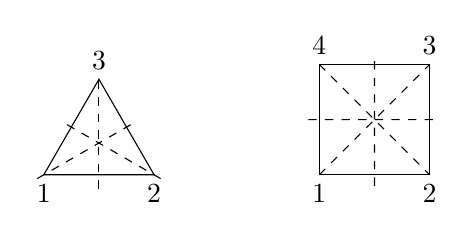
\begin{tikzpicture}[scale=.7]
\draw (0,0)--(2,0)--(1,1.732)--cycle;
\foreach \x/\y/\a/\b in {0/0/1/below,2/0/2/below,1/1.732/3/above}
  \node[\b] at (\x,\y) {$\a$};
\draw[dashed] (1,-.25)--(1,1.73);
\draw[dashed] (-.12,-.07)--(1.65,.95);
\draw[dashed] (2.12,-.07)--(.35,.95);
\begin{scope}[xshift=5cm]
\draw (0,0) rectangle (2,2);
\foreach \x/\y/\a/\b in {0/0/1/below,2/0/2/below,2/2/3/above,0/2/4/above}
  \node[\b] at (\x,\y) {$\a$};
\draw[dashed] (-.2,1)--(2.2,1) (1,-.2)--(1,2.2) (0,0)--(2,2) (0,2)--(2,0);
\end{scope}
\end{tikzpicture}

Gli assi tratteggiati danno le tre riflessioni del triangolo e le quattro del quadrato.
\end{center}

\begin{osservazione}[Sottogruppi diedrali]
Le rotazioni formano il ciclico $\langle r\rangle$. I suoi sottogruppi sono $\langle r^d\rangle$ per $d\mid n$, $d>0$. Ogni riflessione $r^js$ genera un sottogruppo di ordine due, perché $(r^js)^2=r^jr^{-j}=1$. Se un sottogruppo $K$ contiene $r^js$ e $K\cap\langle r\rangle=\langle r^d\rangle$, allora
\[
 K=\langle r^d,r^js\rangle
 =\{r^{td},r^{td+j}s:0\le t<n/d\}.
\]
Infatti il prodotto di una riflessione di $K$ per $r^js$ è una rotazione di $K$, quindi ogni riflessione di $K$ compare nell'elenco. Questo include i sottogruppi $\langle r^d,s\rangle$ delle lezioni.
\end{osservazione}
\Needspace{10\baselineskip}
\begin{esercizio}
Calcolare $Z(S_n)$ per $n\ge3$ e $Z(D_n)$, in particolare per il triangolo e il quadrato.
\end{esercizio}
\begin{svolgimento}
Se $z$ è centrale in $S_n$, allora $(z(i)\ z(j))=(i\ j)$ per ogni trasposizione. Fissato $i$, scegliamo $j,k$ distinti fra loro e da $i$. Ne segue $z(i)\in\{i,j\}\cap\{i,k\}=\{i\}$. Dunque $Z(S_n)=\{1\}$.

In $D_n$ basta commutare con i due generatori. Nessuna riflessione è centrale, perché coniuga $r$ in $r^{-1}\ne r$. La rotazione $r^i$ commuta con $s$ se e solo se $r^i=r^{-i}$, ossia $n\mid 2i$. Per $n$ dispari resta soltanto $1$. Per $n$ pari il centro è $\{1,r^{n/2}\}$, dove il secondo elemento è il mezzo giro. Quindi $Z(D_3)=\{1\}$ e $Z(D_4)=\{1,(1\ 3)(2\ 4)\}$. Benché $D_4\le S_4$, il mezzo giro può essere centrale nel sottogruppo senza esserlo in $S_4$: in generale $Z(G)\cap H\subseteq Z(H)$ per $H\le G$.
\end{svolgimento}

\section{Classi laterali e teorema di Lagrange}
% A–L 23:3–7, 24:1–4; M–Z 23:1–7, 24:1–3.
\begin{definizione}
Per $H\le G$ e $a\in G$, la \textbf{classe laterale destra} $Ha=\{ha:h\in H\}$ si ottiene moltiplicando gli elementi di $H$ a destra per $a$. La \textbf{classe laterale sinistra} è $aH=\{ah:h\in H\}$. In un gruppo abeliano coincidono. In $(\Z,+)$ con $H=m\Z$, $m\ge1$, si ritrovano precisamente le $m$ classi resto $a+m\Z$, $0\le a<m$.
\end{definizione}
\begin{proposizione}
\begin{enumerate}
\item $Ha=Hb$ se e solo se $ab^{-1}\in H$. Per le classi sinistre $aH=bH$ se e solo se $b^{-1}a\in H$.
\item Le classi destre distinte formano una partizione di $G$, come pure le sinistre. Ogni classe ha cardinalità $|H|$.
\end{enumerate}
\end{proposizione}
\begin{proof}
\textbf{1.} Se $Ha=Hb$, allora $a=hb$ per qualche $h\in H$, cioè $ab^{-1}\in H$. Viceversa, se $a=hb$, si ha $Ha=Hhb=Hb$ perché la moltiplicazione per $h$ permuta $H$ con inversa la moltiplicazione per $h^{-1}$. A sinistra lo stesso argomento parte da $a=bh$. Prendendo gli inversi in $H$ si possono anche usare rispettivamente $ba^{-1}$ e $a^{-1}b$. In particolare $Ha=H$ e $aH=H$ precisamente quando $a\in H$. Altrimenti nessuna delle due classi contiene il neutro e quindi nessuna è un sottogruppo.

\textbf{2.} L'uguaglianza $Ha=Hb$ definisce una relazione di equivalenza su $G$. Per il punto 1 la classe di $a$ è $\{b:ba^{-1}\in H\}=Ha$. Il teorema~\ref{teo:partizioni} dà quindi la partizione in classi di equivalenza. A sinistra si procede usando $a^{-1}b\in H$. Le mappe $h\mapsto ha$ e $h\mapsto ah$ sono biezioni da $H$ sulle rispettive classi, con inverse $x\mapsto xa^{-1}$ e $x\mapsto a^{-1}x$.
\end{proof}
L'inversione manda $Ha$ in $a^{-1}H$ e applicata due volte restituisce la classe iniziale. Il numero delle classi destre è dunque quello delle sinistre. Si chiama \textbf{indice} di $H$ in $G$ e si scrive $[G:H]$.
\begin{teorema}[Lagrange]\label{teo:lagrange}
Se $G$ è finito e $H\le G$, allora $|G|=[G:H]|H|$. In particolare $|H|$ divide $|G|$.
\end{teorema}
\begin{proof}
Si scelga un rappresentante per ciascuna classe destra distinta. Le corrispondenti classi sono disgiunte, ricoprono $G$ e contengono ciascuna $|H|$ elementi. Sommando le loro cardinalità si ottiene la formula.
\end{proof}
\begin{esempio}
In $S_3$, per $H=\langle(1\ 2)\rangle$, l'indice è $3$. Oltre a $H$ si hanno
\[
\begin{array}{c|cc}
a&Ha&aH\\\hline
(1\ 3)&\{(1\ 3),(1\ 3\ 2)\}&\{(1\ 3),(1\ 2\ 3)\}\\
(2\ 3)&\{(2\ 3),(1\ 2\ 3)\}&\{(2\ 3),(1\ 3\ 2)\}.
\end{array}
\]
Per $N=\langle(1\ 2\ 3)\rangle$ l'indice è $2$. L'unica classe oltre a $N$, sia a destra sia a sinistra, contiene le tre trasposizioni. In generale, per indice $2$ e $a\notin H$ si ha $Ha=G\setminus H=aH$.
\end{esempio}
\begin{corollario}
\begin{enumerate}
\item In un gruppo finito $\operatorname{ord}(g)\mid |G|$ e $g^{|G|}=1$. Un gruppo di ordine primo è generato da ciascun suo elemento diverso dal neutro.
\item Se $m\ge2$ e $\operatorname{MCD}(a,m)=1$, allora $a^{\varphi(m)}\equiv1\pmod m$ (teorema di Eulero). Per ogni primo positivo $p$ e ogni intero $a$ vale $a^p\equiv a\pmod p$ (piccolo teorema di Fermat).
\end{enumerate}
\end{corollario}
\begin{proof}
\textbf{1.} Applicare Lagrange a $\langle g\rangle$, che ha cardinalità $d=\operatorname{ord}(g)$. Scrivendo $|G|=dq$ segue $g^{|G|}=(g^d)^q=1$. Se $|G|=p$ e $g\ne1$, l'unico divisore possibile per $d>1$ è $p$, quindi $\langle g\rangle=G$.

\textbf{2.} Applicare il punto 1 al gruppo moltiplicativo delle unità modulo $m$, che contiene $[a]_m$ ed ha $\varphi(m)$ elementi. Per $m=p$ primo e $p\nmid a$, moltiplicare $a^{p-1}\equiv1\pmod p$ per $a$. Se $p\mid a$, entrambi i membri di $a^p\equiv a\pmod p$ sono congrui a zero.
\end{proof}
\begin{esempio}[I conversi di Lagrange]
In $S_5$ non esiste alcun sottogruppo di ordine $7$ perché $7\nmid120$. La divisibilità, quando vale, può non bastare. In $S_3$ nessun elemento ha ordine $6$. In $S_4$ gli ordini possibili sono $1,2,3,4$, come si legge dalle partizioni di $4$ in lunghezze di cicli. In particolare manca un elemento di ordine $12$, mentre esiste un sottogruppo di ordine $12$, ossia $A_4$. Anzi tutti i divisori di $24$ sono ordini di sottogruppi: per $1,2,3,4$ bastano i ciclici, per $6$ le permutazioni che fissano $4$, per $8$ il gruppo del quadrato, per $12,24$ i gruppi $A_4,S_4$. Nel caso di un gruppo ciclico finito il converso vale anche per gli elementi, come segue dalla classificazione dei suoi sottogruppi.
\end{esempio}

% !TeX root = ../main.tex
% A–L 24:2–8; M–Z 24:3–9.
\section{Sottogruppi normali e gruppi quoziente}
Una \textbf{congruenza} su $G$ è un'equivalenza $\sim$ compatibile con il prodotto: se $a\sim a'$ e $b\sim b'$, allora $ab\sim a'b'$. È esattamente la condizione perché $[a][b]=[ab]$ sia ben definito. Quali partizioni di un gruppo hanno questa proprietà?
\begin{proposizione}
Per una congruenza su $G$, posto $H=[1]$, si ha:
\begin{enumerate}
\item $H$ è un sottogruppo;
\item $a\sim b\iff Ha=Hb\iff aH=bH$, e in particolare $[a]=Ha=aH$.
\end{enumerate}
\end{proposizione}
\begin{proof}
\textbf{1.} Per riflessività $1\in H$. Se $x,y\sim1$, la compatibilità dà $xy\sim1$. Moltiplicando $x\sim1$ per $x^{-1}$ a destra si ottiene $1\sim x^{-1}$, dunque $x^{-1}\in H$.

\textbf{2.} Moltiplicando $a\sim b$ a destra per $b^{-1}$ si ottiene $ab^{-1}\sim1$, e viceversa basta rimoltiplicare per $b$. Pertanto $a\sim b\iff ab^{-1}\in H\iff Ha=Hb$. Moltiplicando a sinistra per $b^{-1}$ si ottiene il criterio $b^{-1}a\in H\iff aH=bH$. Le due descrizioni della classe di $a$ coincidono.
\end{proof}
\begin{teorema}[Criteri di normalità]
Per un sottogruppo $H$ di $G$ sono equivalenti:
\begin{enumerate}
\item la relazione $Ha=Hb$ è una congruenza;
\item $gH=Hg$ per ogni $g\in G$;
\item la relazione $aH=bH$ è una congruenza;
\item $gHg^{-1}=H$ per ogni $g\in G$;
\item $gHg^{-1}\subseteq H$ per ogni $g\in G$.
\end{enumerate}
In tal caso $H$ si dice \textbf{normale} in $G$ e si scrive $H\trianglelefteq G$.
\end{teorema}
\begin{proof}
\textbf{$1\Rightarrow2$ e $3\Rightarrow2$.} Per entrambe le relazioni la classe del neutro è $H$. La proposizione precedente identifica ogni classe sia con $Hg$ sia con $gH$.

\textbf{$2\Rightarrow1,3$.} Le due relazioni coincidono. Se $a\sim a'$ e $b\sim b'$, allora $ab\sim a'b$ usando le classi destre, perché $(ab)(a'b)^{-1}=aa'^{-1}\in H$. Inoltre $a'b\sim a'b'$ usando le sinistre, perché $(a'b)^{-1}(a'b')=b^{-1}b'\in H$. La transitività dà la compatibilità.

\textbf{$2\Leftrightarrow4\Rightarrow5$.} Moltiplicare $gH=Hg$ a destra per $g^{-1}$, o l'uguaglianza risultante per $g$. L'uguaglianza implica l'inclusione.

\textbf{$5\Rightarrow4$.} Il punto 5 vale anche per $g^{-1}$. Quindi per ogni $h\in H$ si ha $g^{-1}hg\in H$ e $h=g(g^{-1}hg)g^{-1}\in gHg^{-1}$. Questa è l'inclusione mancante.
\end{proof}
Le congruenze su $G$ corrispondono dunque biunivocamente ai suoi sottogruppi normali: da una congruenza si prende la classe del neutro e da $N\trianglelefteq G$ si prende l'uguaglianza delle classi laterali modulo $N$. I due risultati precedenti mostrano che le costruzioni sono inverse.

\begin{definizione}
Il \textbf{gruppo quoziente} è $G/N=\{gN:g\in G\}$ con $(gN)(hN)=(gh)N$. La normalità garantisce l'indipendenza dai rappresentanti. L'associatività viene da quella di $G$, il neutro è $N$ e l'inverso di $gN$ è $g^{-1}N$. La \textbf{proiezione canonica} $\pi:G\to G/N$, $g\mapsto gN$, è un morfismo per la formula del prodotto ed è suriettiva per definizione. È iniettiva precisamente per $N=\{1\}$: la fibra di $N$ è $N$, e nel caso banale tutte le classi sono singoletti.
\end{definizione}
In un gruppo abeliano ogni sottogruppo è normale. In particolare il quoziente additivo di $\Z$ per $m\Z$, $m\ge1$, ha le classi $[0]_m,\ldots,[m-1]_m$. Per indice due le classi destra e sinistra di ogni elemento esterno coincidono col complemento del sottogruppo. Quindi ogni sottogruppo di indice due è normale, in particolare $A_n\trianglelefteq S_n$ per $n\ge2$.

\Needspace{12\baselineskip}
\begin{esercizio}
Stabilire se sono normali $\langle(1\ 2)\rangle$ in $S_3$, $\langle(1\ 2\ 3)\rangle$ in $S_3$ e in $S_4$, e $\langle(1\ 2\ 3\ 4)\rangle$ in $S_4$. Verificare che $V=\{1,(1\ 2)(3\ 4),(1\ 3)(2\ 4),(1\ 4)(2\ 3)\}$ è un sottogruppo normale di $S_4$ contenuto in $A_4$.
\end{esercizio}
\begin{svolgimento}
Il coniugato di $(1\ 2)$ tramite $(2\ 3)$ è $(1\ 3)$, esterno al primo sottogruppo. Il sottogruppo del $3$-ciclo ha indice due in $S_3$, mentre in $S_4$ il coniugio tramite $(1\ 4)$ produce $(4\ 2\ 3)$, che muove $4$. Infine il coniugato di $(1\ 2\ 3\ 4)$ tramite $(1\ 2)$ è $(2\ 1\ 3\ 4)$, diverso sia dal generatore sia dalla sua inversa, le sole potenze di ordine quattro.

In $V$ ciascun elemento non banale è il proprio inverso. Detti $x,y,z$ i tre elementi nell'ordine indicato, il calcolo dà $xy=z$. Invertendo si ha anche $yx=z$, e quindi $xz=zx=y$, $yz=zy=x$. Questo prova la chiusura. La coniugazione permuta le doppie trasposizioni perché conserva la struttura ciclica. Perciò $V$ è normale e la segnatura dei suoi elementi è positiva.
\end{svolgimento}
\Needspace{9\baselineskip}
\begin{esercizio}
Dimostrare che $A_4$ non contiene un sottogruppo di ordine $6$.
\end{esercizio}
\begin{svolgimento}
Un tale $H$ avrebbe indice due. La proiezione su $A_4/H$, di ordine due, manderebbe ogni $3$-ciclo nel neutro: la sua immagine avrebbe cubo uguale al neutro e, per Lagrange, anche quadrato uguale al neutro. Quindi $H$ conterrebbe tutti gli otto $3$-cicli (quattro scelte del punto fisso e due versi), impossibile per $|H|=6$.
\end{svolgimento}

\Needspace{10\baselineskip}
\begin{esercizio}
In $\operatorname{Aff}(\R)$ verificare la normalità delle traslazioni e stabilire se le omotetie centrate nell'origine sono normali. In $D_n$ esaminare $\langle r\rangle$ e $\langle s\rangle$.
\end{esercizio}
\begin{svolgimento}
Per $f(x)=ax+b$, $a\ne0$, e $t_c(x)=x+c$ si ha $ft_cf^{-1}(x)=x+ac$, ancora una traslazione. Invece il coniugato di $x\mapsto2x$ tramite $x\mapsto x+1$ è $x\mapsto2x-1$, che non fissa l'origine. In $D_n$ il sottogruppo delle rotazioni ha indice due. Per $n\ge3$ risulta $rsr^{-1}=r^2s\ne s$, poiché $r^2\ne1$. Questo coniugato è una riflessione diversa da $s$, quindi esterna a $\langle s\rangle$.
\end{svolgimento}
\begin{definizione}
Per un morfismo di gruppi $f:G\to K$, il \textbf{nucleo} è $\ker f=\{g\in G:f(g)=1_K\}=f^*(\{1_K\})$ e l'\textbf{immagine} è $\operatorname{Im}f=\{f(g):g\in G\}$. Per la proiezione canonica si ottengono $\ker\pi=N$ e $\operatorname{Im}\pi=G/N$.
\end{definizione}

